%% Beginning of file 'sample631.tex'
%%
%% Modified 2021 March
%%
%% This is a sample manuscript marked up using the
%% AASTeX v6.31 LaTeX 2e macros.
%%
%% AASTeX is now based on Alexey Vikhlinin's emulateapj.cls 
%% (Copyright 2000-2015).  See the classfile for details.

%% AASTeX requires revtex4-1.cls and other external packages such as
%% latexsym, graphicx, amssymb, longtable, and epsf.  Note that as of 
%% Oct 2020, APS now uses revtex4.2e for its journals but remember that 
%% AASTeX v6+ still uses v4.1. All of these external packages should 
%% already be present in the modern TeX distributions but not always.
%% For example, revtex4.1 seems to be missing in the linux version of
%% TexLive 2020. One should be able to get all packages from www.ctan.org.
%% In particular, revtex v4.1 can be found at 
%% https://www.ctan.org/pkg/revtex4-1.

%% The first piece of markup in an AASTeX v6.x document is the \documentclass
%% command. LaTeX will ignore any data that comes before this command. The 
%% documentclass can take an optional argument to modify the output style.
%% The command below calls the preprint style which will produce a tightly 
%% typeset, one-column, single-spaced document.  It is the default and thus
%% does not need to be explicitly stated.
%%
%% using aastex version 6.3
\documentclass[linenumbers, twocolumn]{aastex631}

%% The default is a single spaced, 10 point font, single spaced article.
%% There are 5 other style options available via an optional argument. They
%% can be invoked like this:
%%
%% \documentclass[arguments]{aastex631}
%% 
%% where the layout options are:
%%
%%  twocolumn   : two text columns, 10 point font, single spaced article.
%%                This is the most compact and represent the final published
%%                derived PDF copy of the accepted manuscript from the publisher
%%  manuscript  : one text column, 12 point font, double spaced article.
%%  preprint    : one text column, 12 point font, single spaced article.  
%%  preprint2   : two text columns, 12 point font, single spaced article.
%%  modern      : a stylish, single text column, 12 point font, article with
%% 		  wider left and right margins. This uses the Daniel
%% 		  Foreman-Mackey and David Hogg design.
%%  RNAAS       : Supresses an abstract. Originally for RNAAS manuscripts 
%%                but now that abstracts are required this is obsolete for
%%                AAS Journals. Authors might need it for other reasons. DO NOT
%%                use \begin{abstract} and \end{abstract} with this style.
%%
%% Note that you can submit to the AAS Journals in any of these 6 styles.
%%
%% There are other optional arguments one can invoke to allow other stylistic
%% actions. The available options are:
%%
%%   astrosymb    : Loads Astrosymb font and define \astrocommands. 
%%   tighten      : Makes baselineskip slightly smaller, only works with 
%%                  the twocolumn substyle.
%%   times        : uses times font instead of the default
%%   linenumbers  : turn on lineno package.
%%   trackchanges : required to see the revision mark up and print its output
%%   longauthor   : Do not use the more compressed footnote style (default) for 
%%                  the author/collaboration/affiliations. Instead print all
%%                  affiliation information after each name. Creates a much 
%%                  longer author list but may be desirable for short 
%%                  author papers.
%% twocolappendix : make 2 column appendix.
%%   anonymous    : Do not show the authors, affiliations and acknowledgments 
%%                  for dual anonymous review.
%%
%% these can be used in any combination, e.g.
%%
%% \documentclass[twocolumn,linenumbers,trackchanges]{aastex631}
%%
%% AASTeX v6.* now includes \hyperref support. While we have built in specific
%% defaults into the classfile you can manually override them with the
%% \hypersetup command. For example,
%%
%% \hypersetup{linkcolor=red,citecolor=green,filecolor=cyan,urlcolor=magenta}
%%
%% will change the color of the internal links to red, the links to the
%% bibliography to green, the file links to cyan, and the external links to
%% magenta. Additional information on \hyperref options can be found here:
%% https://www.tug.org/applications/hyperref/manual.html#x1-40003
%%
%% Note that in v6.3 "bookmarks" has been changed to "true" in hyperref
%% to improve the accessibility of the compiled pdf file.
%%
%% If you want to create your own macros, you can do so
%% using \newcommand. Your macros should appear before
%% the \begin{document} command.
%%
\newcommand{\vdag}{(v)^\dagger}
\newcommand\aastex{AAS\TeX}
\newcommand\latex{La\TeX}
\usepackage{multirow}
\usepackage{fancyvrb}
%% Reintroduced the \received and \accepted commands from AASTeX v5.2
%\received{March 1, 2021}
%\revised{April 1, 2021}
%\accepted{\today}

%% Command to document which AAS Journal the manuscript was submitted to.
%% Adds "Submitted to " the argument.
\submitjournal{ApJ}

%% For manuscript that include authors in collaborations, AASTeX v6.31
%% builds on the \collaboration command to allow greater freedom to 
%% keep the traditional author+affiliation information but only show
%% subsets. The \collaboration command now must appear AFTER the group
%% of authors in the collaboration and it takes TWO arguments. The last
%% is still the collaboration identifier. The text given in this
%% argument is what will be shown in the manuscript. The first argument
%% is the number of author above the \collaboration command to show with
%% the collaboration text. If there are authors that are not part of any
%% collaboration the \nocollaboration command is used. This command takes
%% one argument which is also the number of authors above to show. A
%% dashed line is shown to indicate no collaboration. This example manuscript
%% shows how these commands work to display specific set of authors 
%% on the front page.
%%
%% For manuscript without any need to use \collaboration the 
%% \AuthorCollaborationLimit command from v6.2 can still be used to 
%% show a subset of authors.
%
%\AuthorCollaborationLimit=2
%
%% will only show Schwarz & Muench on the front page of the manuscript
%% (assuming the \collaboration and \nocollaboration commands are
%% commented out).
%%
%% Note that all of the author will be shown in the published article.
%% This feature is meant to be used prior to acceptance to make the
%% front end of a long author article more manageable. Please do not use
%% this functionality for manuscripts with less than 20 authors. Conversely,
%% please do use this when the number of authors exceeds 40.
%%
%% Use \allauthors at the manuscript end to show the full author list.
%% This command should only be used with \AuthorCollaborationLimit is used.

%% The following command can be used to set the latex table counters.  It
%% is needed in this document because it uses a mix of latex tabular and
%% AASTeX deluxetables.  In general it should not be needed.
%\setcounter{table}{1}

%%%%%%%%%%%%%%%%%%%%%%%%%%%%%%%%%%%%%%%%%%%%%%%%%%%%%%%%%%%%%%%%%%%%%%%%%%%%%%%%
%%
%% The following section outlines numerous optional output that
%% can be displayed in the front matter or as running meta-data.
%%
%% If you wish, you may supply running head information, although
%% this information may be modified by the editorial offices.
\shorttitle{ASPIRED toolkit}
\shortauthors{Lam et al.}
%%
%% You can add a light gray and diagonal water-mark to the first page 
%% with this command:
%% \watermark{text}
%% where "text", e.g. DRAFT, is the text to appear.  If the text is 
%% long you can control the water-mark size with:
%% \setwatermarkfontsize{dimension}
%% where dimension is any recognized LaTeX dimension, e.g. pt, in, etc.
%%
%%%%%%%%%%%%%%%%%%%%%%%%%%%%%%%%%%%%%%%%%%%%%%%%%%%%%%%%%%%%%%%%%%%%%%%%%%%%%%%%
\graphicspath{{./}{figures/}}
%% This is the end of the preamble.  Indicate the beginning of the
%% manuscript itself with \begin{document}.

\begin{document}

\title{Automated SpectroPhotometric Image REDuction (\textsc{ASPIRED})}


%% LaTeX will automatically break titles if they run longer than
%% one line. However, you may use \\ to force a line break if
%% you desire. In v6.31 you can include a footnote in the title.

%% A significant change from earlier AASTEX versions is in the structure for 
%% calling author and affiliations. The change was necessary to implement 
%% auto-indexing of affiliations which prior was a manual process that could 
%% easily be tedious in large author manuscripts.
%%
%% The \author command is the same as before except it now takes an optional
%% argument which is the 16 digit ORCID. The syntax is:
%% \author[xxxx-xxxx-xxxx-xxxx]{Author Name}
%%
%% This will hyperlink the author name to the author's ORCID page. Note that
%% during compilation, LaTeX will do some limited checking of the format of
%% the ID to make sure it is valid. If the "orcid-ID.png" image file is 
%% present or in the LaTeX pathway, the OrcID icon will appear next to
%% the authors name.
%%
%% Use \affiliation for affiliation information. The old \affil is now aliased
%% to \affiliation. AASTeX v6.31 will automatically index these in the header.
%% When a duplicate is found its index will be the same as its previous entry.
%%
%% Note that \altaffilmark and \altaffiltext have been removed and thus 
%% can not be used to document secondary affiliations. If they are used latex
%% will issue a specific error message and quit. Please use multiple 
%% \affiliation calls for to document more than one affiliation.
%%
%% The new \altaffiliation can be used to indicate some secondary information
%% such as fellowships. This command produces a non-numeric footnote that is
%% set away from the numeric \affiliation footnotes.  NOTE that if an
%% \altaffiliation command is used it must come BEFORE the \affiliation call,
%% right after the \author command, in order to place the footnotes in
%% the proper location.
%%
%% Use \email to set provide email addresses. Each \email will appear on its
%% own line so you can put multiple email address in one \email call. A new
%% \correspondingauthor command is available in V6.31 to identify the
%% corresponding author of the manuscript. It is the author's responsibility
%% to make sure this name is also in the author list.
%%
%% While authors can be grouped inside the same \author and \affiliation
%% commands it is better to have a single author for each. This allows for
%% one to exploit all the new benefits and should make book-keeping easier.
%%
%% If done correctly the peer review system will be able to
%% automatically put the author and affiliation information from the manuscript
%% and save the corresponding author the trouble of entering it by hand.

%\correspondingauthor{August Muench}
%\email{greg.schwarz@aas.org, gus.muench@aas.org}

\author[0000-0002-9347-2298]{Marco C. Lam}
\affiliation{School of Physics and Astronomy, Tel Aviv University, Tel Aviv 69978, Israel}
\affiliation{Astrophysics Research Institute, Liverpool John Moores University, IC2, LSP, 146 Brownlow Hill, Liverpool L3 5RF, UK}
\affiliation{Astronomical Observatory, University of Warsaw, Al. Ujazdowskie 4, 00-478, Warszawa, Poland}

\author[0000-0003-3434-1922]{Robert J. Smith}
\affiliation{Astrophysics Research Institute, Liverpool John Moores University, IC2, LSP, 146 Brownlow Hill, Liverpool L3 5RF, UK}

\author[0000-0001-7090-4898]{Iair Arcavi}
\affiliation{School of Physics and Astronomy, Tel Aviv University, Tel Aviv 69978, Israel}
\affiliation{CIFAR Azrieli Global Scholars program, CIFAR, Toronto, Canada}

\author[0000-0001-8397-5759]{Iain A. Steele}
\affiliation{Astrophysics Research Institute, Liverpool John Moores University, IC2, LSP, 146 Brownlow Hill, Liverpool L3 5RF, UK}

\author[0000-0003-2780-7843]{Josh Veitch-Michaelis}
\affiliation{Astrophysics Research Institute, Liverpool John Moores University, IC2, LSP, 146 Brownlow Hill, Liverpool L3 5RF, UK}
\affiliation{Department of Physics and Wisconsin IceCube Particle Astrophysics Center, University of Wisconsin, Madison, WI 53706, USA}
\affiliation{ETH Z\"urich, Systems Group, Stampfenbachstrasse 114, 8092 Z\"urich, Switzerland}

\author[0000-0002-9658-6151]{Lukasz Wyrzykowski}
\affiliation{Astronomical Observatory, University of Warsaw, Al. Ujazdowskie 4, 00-478, Warszawa, Poland}


%% Note that the \and command from previous versions of AASTeX is now
%% depreciated in this version as it is no longer necessary. AASTeX 
%% automatically takes care of all commas and "and"s between authors names.

%% AASTeX 6.31 has the new \collaboration and \nocollaboration commands to
%% provide the collaboration status of a group of authors. These commands 
%% can be used either before or after the list of corresponding authors. The
%% argument for \collaboration is the collaboration identifier. Authors are
%% encouraged to surround collaboration identifiers with s. The 
%% \nocollaboration command takes no argument and exists to indicate that
%% the nearby authors are not part of surrounding collaborations.

%% Mark off the abstract in the ``abstract'' environment. 
\begin{abstract}
%%%%%%%%%%%%%%%%%%%%%%%%%%%%%%%%%%%%%%%%%%%%%%%%%%%%%%%%%%%%%%%%%%%%%%%%%%%%%%%%
We provide a suite of public open-source spectral data reduction software to
rapidly obtain scientific products from all forms of long-slit-like
spectroscopic observations. Automated SpectroPhotometric
REDuction~(\textsc{ASPIRED}) is a \textsc{Python}-based spectral data
reduction toolkit. It is designed to be a general toolkit with high flexibility
for users to refine and optimize their data reduction routines for the
individual characteristics of their instruments. The default configuration is
appropriate for use on a low-resolution long-slit spectrometer at a quick-look
quality. \textcolor{red}{Some moderate one-off effort in modifying the
configuration will allow repeatable science-ready reduced spectral data}
from a \textcolor{red}{reduced image}. More fine-tuning and extra (pre-)processing can
extend the reduction to systems with more complex setups. We compare some
example spectra reduced with \textsc{ASPIRED} to published data processed with
\textsc{iraf}-based and \textsc{STARLINK}-based pipelines, and find no loss in
the quality of the final product. The \textsc{Python}-based \textsc{iraf}-free
\textsc{ASPIRED} can significantly ease the effort of an Astronomer in
constructing their own data reduction workflow, enabling simpler solutions to
data reduction automation. This availability of near real-time science-ready
data will allow adaptive observing strategies, particularly important in, but
not limited to, time-domain astronomy.
\end{abstract}

%% Keywords should appear after the \end{abstract} command. 
%% The AAS Journals now uses Unified Astronomy Thesaurus concepts:
%% https://astrothesaurus.org
%% You will be asked to selected these concepts during the submission process
%% but this old "keyword" functionality is maintained in case authors want
%% to include these concepts in their preprints.
\keywords{}

%% From the front matter, we move on to the body of the paper.
%% Sections are demarcated by \section and \subsection, respectively.
%% Observe the use of the LaTeX \label
%% command after the \subsection to give a symbolic KEY to the
%% subsection for cross-referencing in a \ref command.
%% You can use LaTeX's \ref and \label commands to keep track of
%% cross-references to sections, equations, tables, and figures.
%% That way, if you change the order of any elements, LaTeX will
%% automatically renumber them.
%%
%% We recommend that authors also use the natbib \citep
%% and \citet commands to identify citations.  The citations are
%% tied to the reference list via symbolic KEYs. The KEY corresponds
%% to the KEY in the \bibitem in the reference list below. 


\section{Introduction}
%%%%%%%%%%%%%%%%%%%%%%%%%%%%%%%%%%%%%%%%%%%%%%%%%%%%%%%%%%%%%%%%%%%%%%%%%%%%%%%%
With major global investments in multi-wavelength and multi-messenger surveys,
time-domain astronomy is entering a golden age. In order to maximally exploit
discoveries from these facilities, rapid spectroscopic follow-up observations
of transient objects~(e.g.,\ supernovae, gravitational-wave optical counterparts
etc.) are needed to provide crucial {\em astrophysical} interpretations. 

Part of
the former OPTICON\footnote{\url{https://www.astro-opticon.org}; now the
OPTICON-RadioNet Pilot \url{https://www.orp-h2020.eu}} project coordinates the
operation of a network of largely self-funded European robotic and conventional
telescopes, collating common science goals and providing the tools to deliver
science-ready photometric and spectroscopic data in near real-time. The goal is
to facilitate automated or interactive decision-making, allowing ``on-the-fly''
modification of observing strategies and rapid triggering of other facilities.
As part of the network's activity, a software development work package was
commissioned under the working title of Automated SpectroPhotometric
REDuction~(\textsc{ASPIRED}), coordinated on
\textsc{Github}\footnote{\url{https://github.com/cylammarco/ASPIRED}}.

%%%%%%%%%%%%%%%%%%%%%%%%%%%%%%%%%%%%%%%%%%%%%%%%%%%%%%%%%%%%%%%%%%%%%%%%%%%%%%%%
The ``industrial standard'' of spectral and image reduction is undoubtedly
the \textsc{iraf} framework~\citep{1986SPIE..627..733T, 1993ASPC...52..173T}.
It has powered many reduction engines in the past and present. However,
unfortunately, \textcolor{red}{the National Optical Astronomy Observatory 
discontinued the support of the software in 2013}, and it is now
entirely relying on community support\footnote{\url{https://iraf-community.github.io}}.
The \textsc{STARLINK}
library\footnote{\url{https://STARLINK.eao.hawaii.edu/STARLINK}} \citep{2014ASPC..485..391C, 2022ASPC..532..559B}
includes substantial resources for data reduction tasks in the \textsc{Figaro} package. It was first initiated
in 1980 under the STARLINK Project, which became defunct in 2005, but the
software survived, and its maintenance effort has since transferred to the
East Asian Observatory. It also comes with a \textsc{Python}
wrapper\footnote{\url{https://github.com/STARLINK/STARLINK-pywrapper}}
to enable low-level code access from high-level programs. These software tools
have made significant contributions to the entire Astrophysics community. They
are very often overlooked when they are so deeply embedded into many systems,
and users do not interact directly with them in this era of big data
and high data rates. However, \textcolor{red}{this is not always the case,
many smaller facilities and individual users are still required to commission
their own data reduction routines, and university students are still learning
data reduction methods from the fundamentals up. These powerful libraries and
tools} also come with a few drawbacks; the most notable obstacle concerns the
ease of installation and linkage of libraries that users often find difficult.

%%%%%%%%%%%%%%%%%%%%%%%%%%%%%%%%%%%%%%%%%%%%%%%%%%%%%%%%%%%%%%%%%%%%%%%%%%%%%%%%
In this generation of user-side Astronomy data handling and processing, as
well as the emphasis in computing courses for scientists, \textsc{Python} is
among the most popular languages due to its ease to use with a shallow learning
curve, readable syntax and simple way to ``glue'' different pieces of software
together. Its flexibility to serve as a scripting and an object-oriented
language makes it useful in many use cases: developing visual tools
with little overhead, prototyping, web-serving, and compiling if
desired. While this broad range of functionality and high-level usage make it
relatively inefficient. \textsc{Python} is an excellent choice of
language for building wrappers on top of highly efficient and well-established codes.
Some of the most used packages, \textsc{scipy}~\citep{2020SciPy-NMeth}
and \textsc{numpy}~\citep{2020NumPy-Array}, are written in \textsc{Fortran}
and \textsc{C}, respectively, to deliver high performance. Multi-threading
and multi-processing are also possible with built-in and other third-party
packages, such as \textsc{mpi4py}~\citep{DALCIN20111124}. 

%%%%%%%%%%%%%%%%%%%%%%%%%%%%%%%%%%%%%%%%%%%%%%%%%%%%%%%%%%%%%%%%%%%%%%%%%%%%%%%%
Various efforts are being made to develop software for the current and
next-generation spectral data reduction. For example,
\textsc{PypeIt}~\citep{pypeit:zenodo, 2020JOSS....5.2308P} is designed for
tailor-made reduction for a range of instruments, and
\textsc{PyReduce}~\citep{2021A&A...646A..32P} is designed for optimal Echelle
spectral reduction (but \textcolor{red}{only handle sky subtraction if a sky frame is provided}). In the \textsc{Astropy}
`Universe'~\citep{astropy:2013, astropy:2018},
\textsc{specreduce}\footnote{\url{https://github.com/astropy/specreduce}}~\citep{pickering_timothy_2022_7007991} is likely to be the
next-generation user-focused data reduction package, but it is still in early
stages of deployment at the time of writing.
\textsc{pyDIS}\footnote{\url{https://github.com/StellarCartography/pydis}} has
all the essential ingredients for reducing spectra but has been out of
maintenance since 2019, and \textsc{specutils}
handles spectral analysis and manipulation but not the reduction itself.

%%%%%%%%%%%%%%%%%%%%%%%%%%%%%%%%%%%%%%%%%%%%%%%%%%%%%%%%%%%%%%%%%%%%%%%%%%%%%%%%
In \textsc{ASPIRED}, we have a different vision of how and what should be
abstracted from the users. Instead of providing a ready-to-go ``black box''
suited for a specific instrument or observations made under particular conditions,
we provide a toolkit that is as general as possible for users to have a set of
high-level data reduction building blocks to process the data in the ways most
appropriate to their instruments and observations. This shifts more of the work
and maintenance to the user-end, but allows rapid modification of the
data reduction workflow to any changes in the instrumental
configuration (such as a detector being refitted, or the detector plane
shifted and rotated by a few pixels during engineering work) and to new instruments. \textsc{ASPIRED}
is thus especially useful for works that repeatedly make use of multiple
spectrographs requiring rapid follow-ups.
Using \textsc{ASPIRED} only requires basic coding skills acquired by most
graduate-level astronomers.

%%%%%%%%%%%%%%%%%%%%%%%%%%%%%%%%%%%%%%%%%%%%%%%%%%%%%%%%%%%%%%%%%%%%%%%%%%%%%%%%
We use the SPRAT spectrograph \citep{2014SPIE.9147E..8HP} mounted on the \textit{Liverpool Telescope}~(\textit{LT}) as our
``first-light'' instrument for development. \textsc{ASPIRED} is currently used
\textcolor{red}{by the transient science research group at the Tel Aviv University
for a proprietary spectral data reduction pipeline of the FLOYDS instrument of
the Las Cumbres Observatory. It is also known to be used}
for quicklook reduction of data obtained by the MISTRAL spectrograph
mounted on the \textit{1.93\,m telescope} at the Observatoire de
Haute-Provence\footnote{\url{http://www.obs-hp.fr/guide/mistral/MISTRAL_spectrograph_camera.shtml}}.
However, as mentioned, we aim to allow high-level tools for users to build and
fine-tune their pipelines to support a wide range of
configurations~\citep{2020arXiv201203505L, marco_2021_4463569}. As of the time
of writing, we have successfully used \textsc{ASPIRED} to reduce data from the
\textit{William Herschel Telescope} Intermediate-dispersion Spectrograph and
Imaging System\footnote{\url{https://www.ing.iac.es/astronomy/instruments/isis}}~(\textit{WHT}/ISIS)
and the Auxiliary-port CAMera~\citep[ACAM;][]{2008SPIE.7014E..6XB}, Las Cumbres
Observatory FLOYDS~\citep[Las Cumbres/FLOYDS;][]{2013PASP..125.1031B}, Gemini Observatory
Gemini Multi-Object Spectrographs long-slit
mode~\citep[Gemini/GMOS-LS;][]{2004PASP..116..425H}, \textit{Gran Telescopio Canarias}
Optical System for Imaging and low-Intermediate-Resolution Integrated
Spectroscopy~\citep[GTC/OSIRIS;][]{2000SPIE.4008..623C},  \textit{Telescopio
Nazionale Galileo} Device Optimised for the LOw
RESolution\footnote{\url{http://www.tng.iac.es/instruments/lrs}}~\citep[\textit{TNG}/DOLORES;][]{1999ldss.work..157M},
the \textit{Very Large Telescope} FOcal Reducer/low dispersion Spectrograph 2~(\textit{VLT}/FORS2); and the \textit{Southern Astrophysical Research Telescope} Goodman High Throughput Spectrograph~\citep[\textit{SOAR}/GHTS][]{2004SPIE.5492..331C}.
We show examples of these reductions in Section~\ref{sec:examples}\footnote{See
also \url{https://github.com/cylammarco/aspired-example}}, and an excert of
example codes in Appendix~\ref{sec:appendix}.

%%%%%%%%%%%%%%%%%%%%%%%%%%%%%%%%%%%%%%%%%%%%%%%%%%%%%%%%%%%%%%%%%%%%%%%%%%%%%%%%
This article is organized as follows: Section \textsection\ref{sec:development}
covers the development and organization of the software. Then, we discuss the
details of the spectral image reduction procedures in Sections~\textsection
\ref{sec:image_reduction} and \ref{sec:spectral_reduction}. In
Section~\textsection{\ref{sec:examples}} we show a few example spectra and
compare then with published reductions.
Section~\textsection{\ref{sec:distribution}}
explains how \textsc{ASPIRED} can be installed and finally in 
Section~\textsection\ref{sec:summary}, we summarize and discuss future
plans.

%%%%%%%%%%%%%%%%%%%%%%%%%%%%%%%%%%%%%%%%%%%%%%%%%%%%%%%%%%%%%%%%%%%%%%%%%%%%%%%%
This article is not intended to serve as an API document\footnote{\url{https://aspired.readthedocs.io/en/latest}\label{rtd}}, nor as a review of the
various methods concerning spectral extraction. Only the high-level
descriptions and the scientific and mathematical technicalities that are
important to the data reduction processes are discussed here.

%%%%%%%%%%%%%%%%%%%%%%%%%%%%%%%%%%%%%%%%%%%%%%%%%%%%%%%%%%%%%%%%%%%%%%%%%%%%%%%%
\section{Development and Structure of \textsc{ASPIRED}}
\label{sec:development}

One of the development goals of \textsc{ASPIRED} is to design a piece of
software that is as modular and portable as possible, \textcolor{red}{such that
it is operable on \textsc{Linux}, \textsc{Mac} and \textsc{Windows} systems. The
last is particularly important as software for Astronomy and Astrophysics are
strongly leaning towards Unix systems, however, \textsc{Windows} has the highest
market share worldwide; furthermore, demographically it is the common choice
among university systems, students and lower-income countries. On top of that,
it is designed to rely} on as few external dependencies as possible.
The ones we do use are those that would require a substantial programming effort to reproduce and have a
proven track record of reliability and/or plan to remain maintained in the
foreseeable future. The explicit top-level dependencies are --
\textsc{astroscrappy}~\citep{curtis_mccully_2018_1482019, 2001PASP..113.1420V}
\textsc{Astropy}~\citep{astropy:2013, astropy:2018},
\textsc{ccdproc}~\citep{matt_craig_2017_1069648},
\textsc{numpy}~\citep{2020NumPy-Array}
\textsc{plotly}~\citep{plotly},
\textsc{rascal}~\citep{2020ASPC..527..627V},
\textsc{scipy}~\citep{2020SciPy-NMeth},
\textsc{spectres}~\citep{2017arXiv170505165C},
\textsc{specutils}, and
\textsc{statsmodels}~\citep{seabold2010statsmodels}. 

We host our source code on \textsc{Github}, which provides version control and other
utilities to facilitate the development. It uses \textsc{git}\footnote{\url{https://git-scm.com}},
issue and bug tracking, high-level project management, and automation with \textsc{Github Actions}
upon each \texttt{commit} for:

\begin{enumerate}
    \item Continuous Integration~(CI) to install the software on \textsc{Linux},
    \textsc{Mac} and \textsc{Windows} systems, and then perform unit tests with
    \textsc{pytest}~\citep{pytest6.2} over most of the functions in multiple
    versions of \textsc{Python};
    \item Generating test coverage reports with \textsc{Coveralls}\footnote{\url{    https://coveralls.io/github/cylammarco/ASPIRED}} which identifies lines in
    the source code that are missed from the tests to assist us in maximising the test coverage;
    \item Continuous Deployment~(CD) through \textsc{PyPI}\footnote{\url{https://pypi.org/project/aspired}} that allows immediate availability of the
    latest numbered version;
    \item Version tracking of the depending packages with 
    \textsc{Dependabot}\footnote{\url{https://dependabot.com}} to stay up to date with external dependencies (a
    pull request is generated automatically and the software is
    tested upon any update of the dependencies); and
    \item Generating API documentation powered by \textsc{Sphinx}\footnote{\url{https://www.sphinx-doc.org/en/master}} which scans for the \textit{decorators}
    and automatically formats the written documentation (docstrings) into
    interactive html pages which can also be exported as a PDF file, and are
    hosted on Read the Docs$^{\ref{rtd}}$.
\end{enumerate}

%%%%%%%%%%%%%%%%%%%%%%%%%%%%%%%%%%%%%%%%%%%%%%%%%%%%%%%%%%%%%%%%%%%%%%%%%%%%%%%%
The initial work package divided the project broadly into three high-level
independent components, which we now detail.

%%%%%%%%%%%%%%%%%%%%%%%%%%%%%%%%%%%%%%%%%%%%%%%%%%%%%%%%%%%%%%%%%%%%%%%%%%%%%%%%
\subsubsection*{Graphical User Interface\\(not in active development)}
In the beginning, we commissioned a prototype of the graphical user
interface\footnote{\url{https://github.com/cylammarco/gASPIRED}} with
\textsc{Electron}\footnote{\url{https://www.electronjs.org}}, which wraps on
top of \textsc{ASPIRED} without needing to adapt the code. Such a setup works seamlessly
for a few reasons: first, \textsc{Python} is an interpreter, it can
execute in run time. It is hence straightforward to run a \textsc{Python}-server to
interact with an \textsc{Electron} instance; second,
\textsc{Plotly}\footnote{\url{https://plotly.com}} has a good balance in
generating interactive and static plots, it requires little effort to interact
with both \textsc{Python} and \textsc{Electron}; third, there is a
\textsc{JavaScript} version of
\textsc{SAOImageDS9}\footnote{\url{https://sites.google.com/cfa.harvard.edu/saoimageds9}}, \textsc{JS9},
that allows rapid and easy interactive image manipulation with an interface
that Astronomers are accustomed to~\citep{2003ASPC..295..489J, eric_mandel_2022_6675771}.
\textsc{Electron} and \textsc{JS9} work like a web service; this prototype also
shows that an \textsc{ASPIRED} graphical user
interface can be deployed as an online tool. Such a high level of
interactivity is, however, no longer in active development and is only served
as a one-off technology demonstrator of its capability.

%%%%%%%%%%%%%%%%%%%%%%%%%%%%%%%%%%%%%%%%%%%%%%%%%%%%%%%%%%%%%%%%%%%%%%%%%%%%%%%%
\subsubsection*{Arc fitting for the Pixel-Wavelength relation (a concurrent development)}

The wavelength calibration process involves identifying distinctive emission
lines from an arc lamp spectrum, to which a function such as a polynomial can be
fit to map the pixel position to the wavelength value. Manual calibration is
straightforward but tedious: first, a user has to locate the peaks of an arc
spectrum in pixel space. Then, they have to assign a wavelength to each peak
based on the emission lines present from the element(s) of the arc lamp.
\textcolor{red}{
Finally, the function to map pixel values to a set of wavelengths is found. Typically a list of known strong calibration lines is used, as provided by the instrument operators in the form of an atlas or a template calibration spectrum. Automation via template matching is a viable, and commonly used, approach for spectral calibration if the instrument configuration is stable~\citep{2020JOSS....5.2308P}. However, this introduces a strong dependency on instrument-specific properties (such as the
}vacuum/contamination condition of the lamp, the combination of elements in the
lamp, the vignetting on the focal plane, the response as a function of wavelength
across the detector, and saturation issues). There is also noise in peak finding routines, for
example, due to detector noise or quantization~(e.g.\ not using sub-pixel peak
finding), as well as complications due to blended lines. \textcolor{red}{
Providing a general, template-free, tool for such a purpose for a range of
specifications is far from easy, but would be much more flexible for cases when
templates are unavailable or the instrument configuration changes often.}

In \textsc{ASPIRED}, the wavelength calibration module is powered by the
RANSAC~(RANdom SAmple Consensus) Assisted Spectral CALibration ~(\textsc{rascal},
\citealt{2020zndo...4117517V, 2020ASPC..527..627V}, Veitch-Michaelis \& Lam in prep.)
library; a concurrent software development project.
\textcolor{red}{\textsc{rascal} does not require templates and is designed to
work with an arbitrary instrument configuration. Users are only
required to supply a list of calibration
lines~(wavelengths), a list of peaks~(pixels), and some knowledge~(e.g.\ minimum
and maximum wavelength limits) of the system to obtain the most appropriate
pixel-to-wavelength solution. \textsc{rascal} builds on the work by \citet{2018ApOpt..57.6876S}, which
searches only for \textit{plausible} sets of arc line/peak correspondences
that follow a linear relation to first order.} RANSAC~\citep{fischler_bolles_1981}
is used to fit a higher-order polynomial model to the candidate correspondences
robustly. \textsc{rascal} extends this strategy to consider the top $N$ sets
of linear relations simultaneously: for each peak~(pixel), the most common
best-fit atlas line~(wavelength) is chosen from those $N$ subsets that have
a merit function better than a given threshold. This acts like a piece-wise
linear fit and allows us to extract most of the correct matches from both the
red and blue ends of the spectrum that was
\textcolor{red}{not possible with \citet{2018ApOpt..57.6876S}}.

%%%%%%%%%%%%%%%%%%%%%%%%%%%%%%%%%%%%%%%%%%%%%%%%%%%%%%%%%%%%%%%%%%%%%%%%%%%%%%%%
\subsubsection*{Data Reduction and Other Calibrations\\(this work)}
This is the core of \textsc{ASPIRED}, which mainly handles the spectral
extraction and calibration processes. At the user level, the software is
organized into two main parts -- \texttt{image\_reduction} and
\texttt{spectral\_reduction}. They are designed to be as modular as possible.
Users are free to use third-party reduction tools to perform part(s) of 
the reduction process and return to continue the reduction with
\texttt{image\_reduction} and \texttt{spectral\_reduction}.

In addition, the data structure class \texttt{SpectrumOneD} handles the
data and metadata of the extracted information. It provides a uniform format
to store the metadata and the extracted data throughout the entire spectral
extraction process. Since multiple spectra can be extracted from a
\texttt{TwoDSpec} object~(e.g.\ extended target or multiple targets aligned on
the slit), each extracted spectrum is stored in an independent
\texttt{SpectrumOneD} object which gets passed from a \texttt{TwoDSpec} object.
In Astronomy, the handling of observational
data is almost exclusively done with FITS files, but they are not
human-readable. In view of that, \textsc{ASPIRED} provides \textcolor{red}{input
and output handling of FITS files, and output in CSV format.} All the
higher-level functions are wrappers on top of a \texttt{spectrumOneD} object.

%%%%%%%%%%%%%%%%%%%%%%%%%%%%%%%%%%%%%%%%%%%%%%%%%%%%%%%%%%%%%%%%%%%%%%%%%%%%%%%%
\section{Image Reduction}
\label{sec:image_reduction}

\textcolor{red}{\textsc{ASPIRED} only intends to provide image reduction methods
for bias, dark and flat corrections. It is } sufficient for simple instrumental
setups, which are the primary targets of \textsc{ASPIRED}.
For example, a long-slit spectrograph with a rectilinear
two-dimensional spectrum illuminated on the detector plane, i.e. the dispersion
and spatial directions are perfectly perpendicular to each other across the
entire detector plane.
\textcolor{red}{In systems with more complex optical design, for example,
instruments have multiple non-parallel spectra illuminated on the
detector plane, \textsc{ASPIRED} is not immediately usable. Extra image
manipulation is needed to further reduce the data into simpler forms that
\textsc{ASPIRED} can handle. In the FLOYDS reduction example below, we
demonstrate that it is possible to extract two non-parallel curved spectra
from a single two-dimensional image. This is possible only because the two
spectra do not cross-contaminate, and thus can be cleanly separated by
applying masks to the data.}

This module allows mean-, median-, and sum-combining, subtracting and dividing
by dark, bias and flat frames. The FITS header of the \textit{first}
light frame provided is retained in the reduced product, while the headers
from the other frames are not stored -- only the file paths are appended to
the end of the FITS header. The FITS file is defaulted to contain an empty
\texttt{PrimaryHDU} with the process data stored in the first
\texttt{ImageHDU} extension as recommended in the FITS Standard 
document\footnote{\url{https://fits.gsfc.nasa.gov/fits_documentation.html}},
but it can also be stored directly in the \texttt{PrimaryHDU} as most users
opt for. Many forms of interactive and static images can be exported,
powered by the \textsc{Plotly} image renderer.

This module only allows basic image reduction, users have to rely on third-party
software to correct for any other effects before continuing the
reduction with \texttt{spectral\_reduction}.

%%%%%%%%%%%%%%%%%%%%%%%%%%%%%%%%%%%%%%%%%%%%%%%%%%%%%%%%%%%%%%%%%%%%%%%%%%%%%%%%
\section{Spectral Reduction}
\label{sec:spectral_reduction}

In the highest-level terms, \textsc{ASPIRED}'s spectral reduction procedures
after image reduction include: (1) identifying and tracing the spectrum(a),
(2) correcting for image distortion, (3) extracting the spectrum(a),
(4) performing wavelength calibration of the science target and a standard
star, (5) computing the sensitivity function using the standard star,
(6) performing atmospheric extinction correction, and finally (7) removing
the telluric absorption features, (8) resampling, and (9) exporting the data.
We omit a few other processes which we believe should be considered as part of
the post-extraction processes or spectral analysis and manipulation. There are
many sophisticated  software packages with good and long track records to
handle these processes post hoc. For example, sky glow subtraction with
\textsc{Skycorr}~\citep{2014A&A...567A..25N}, or telluric
absorption removal without supplementary calibration data with
\textsc{MoleFit}~\citep{2015A&A...576A..77S, 2015A&A...576A..78K}.

The \texttt{spectral\_reduction} is a large module that covers both the
two-dimensional and one-dimensional operations through the \texttt{TwoDSpec} and
\texttt{OneDSpec} classes, respectively. The former provides image
rectification, spectral tracing, spectral extraction of the target and the
arc, and locating the peaks of the arc lines. The latter performs
wavelength calibration (with the \texttt{WavelengthCalibration} class),
flux calibration (with the \texttt{FluxCalibration} class), atmospheric
extinction correction, \textcolor{red}{telluric absorption correction, and
spectral resampling.} Diagnostic images can be exported at each step of the
two- and one-dimensional operations. This also includes the wavelength
calibration diagnostic that wraps around \textsc{rascal} and uses their native
plotting capability. Since the flux calibration has to be performed
with a standard star spectrum, it is necessary for the \texttt{OneDSpec}
object to have information on both the target and the standard one-dimensional
spectra. Thus, a \texttt{OneDSpec} object keeps a dictionary of lists: --
\texttt{science\_spectrum\_list} and \texttt{standard\_spectrum\_list}. At the
time of writing, \textsc{ASPIRED} only supports wavelength calibration from one (total
stacked) arc frame and flux calibration from one (total stacked) standard star frame.

The following describes the technical details of the nine reduction steps mentioned above.
We use the following convention throughout this article: the spectral image is
dispersed on the detector plane such that the left side~(small pixel number)
corresponds to the blue part of the spectrum and the right side~(large pixel
number) to the red part in the dispersion direction, while the direction
perpendicular to it is the spatial direction.

\texttt{spectral\_reduction} accepts images that are rotated or flipped
compared to the description above, but extra arguments have to be provided
in the initialisation step to set the data into the orientation as defined
above.

%%%%%%%%%%%%%%%%%%%%%%%%%%%%%%%%%%%%%%%%%%%%%%%%%%%%%%%%%%%%%%%%%%%%%%%%%%%%%%%%
\subsection{Spectral Identification and Tracing}
\label{sec:tracing}
Conventionally, to obtain the position of a spectrum in a frame~(i.e.\ trace),
the center of the spectrum in the dispersion direction is first identified. Then
a choice of algorithm scans across the spectral image to identify
the spectral position over the entire dispersion direction. In \textsc{ASPIRED},
the \texttt{ap\_trace} function works by dividing the two-dimensional spectrum
into sub-spectra. Then each part is summed along the dispersion direction
before cross-correlating with the adjacent sub-spectra, using an optional variable
scaling factor that models a linear change in the width of the trace (this optional scaling factor is turned off by default). This allows both the shift and the scaling of
the spectrum(a) along the dispersion direction to be found simultaneously. The
middle of the two-dimensional spectrum is used as the zero point of the
procedure. This tracing procedure is illustrated in Figure \ref{fig:trace}, and described in more detail here:
\begin{enumerate}
    \item
        The input two-dimensional spectrum is divided into \texttt{nwindow}
        overlapping sub-spectra.
    \item
        Each sub-spectrum is summed along the dispersion direction
        in order to improve the signal(s) of the spectrum(a) along
        the spatial direction to generate the line spread function
        of that subspectrum.
    \item
        Each line spread function is upscaled by a factor of
        \texttt{resample\_factor} to allow for sub-pixel correlation
        precision. This utilises the \texttt{scipy.signal.resample}
        function to fit the spatial profile with a cubic spline.
    \item
        The $i$-th line spread function is then cross-correlated to the $i+1$-th
        line spread function. The shift and scale correspond to the maximum
        correlation within the tolerance limit, \texttt{tol}, and are stored.
    \item
        The shifts relative to the central sub-spectrum are used to
        fit for a polynomial solution with a constant arbitrary offset.
    \item
        While the spatial spectra are cross-correlated, they are also
        aligned and stacked to find the peak of the line spread profile.
        Peak finding is performed with \texttt{scipy.signal.find\_peaks}
        and returns the list of peaks sorted by their prominence, which is
        defined as the maximum count of the peak subtracted by the local
        background. The total stacked line spread profile is fitted with
        a Gaussian function to get the spread of the spectrum~(standard
        deviation). This would not be used in the case of top-hat
        extraction~(see section \textsection\ref{sec:tophat}).
\end{enumerate}

Manually supplying a trace (determined a priori or copied from another observation) is possible with the \texttt{add\_trace}
function. This is particularly useful for faint and/or confused
sources that are beyond the capability of automated tracing. For
example, if there is a faint transient source on top of a galaxy,
a manual offset may be needed for extraction if the host is
dominating the flux to a level that forced extraction is necessary.
For an optical design where the source spectrum is always illuminated
at the same pixels of a detector, it is possible to reuse the trace
from the standard frame for spectral extraction of the science target.

\begin{figure}
    \centering
    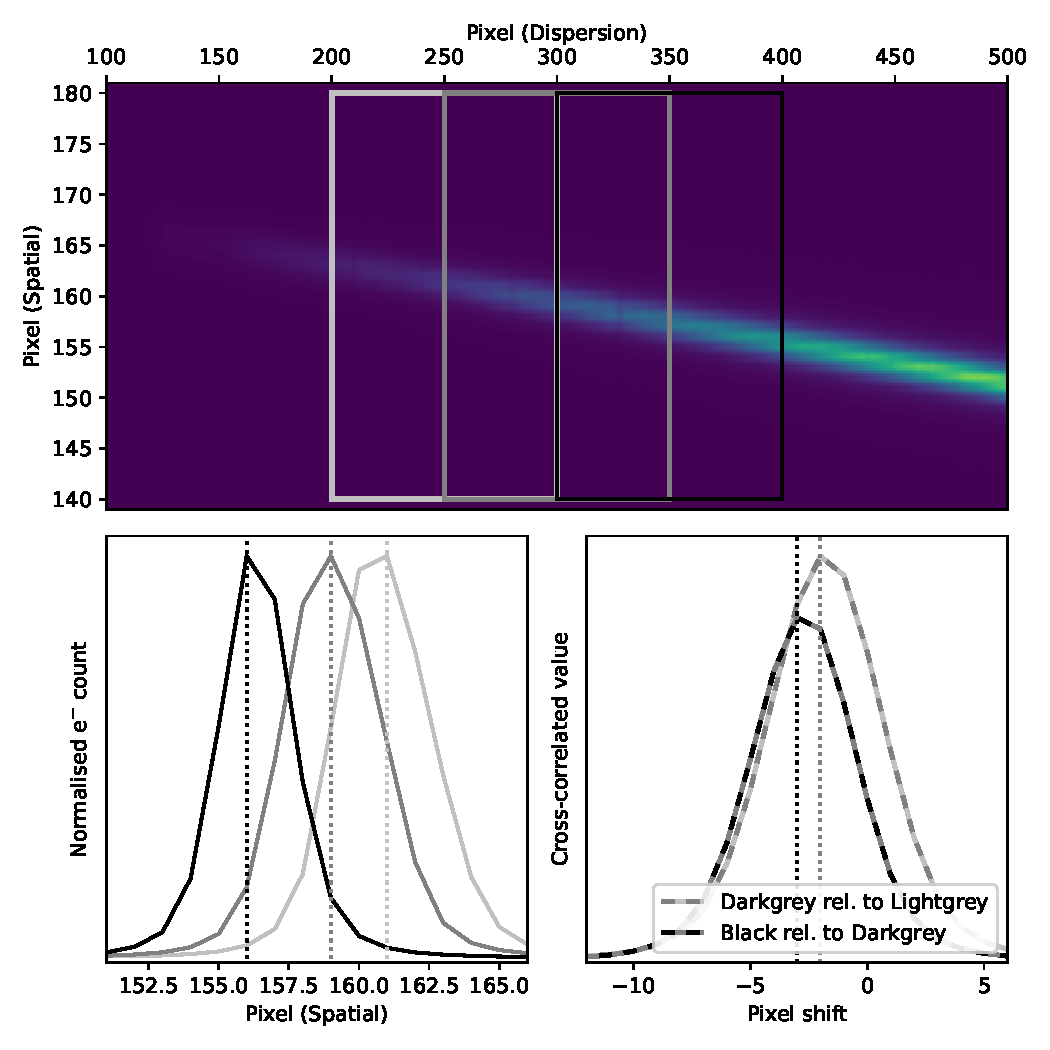
\includegraphics[width=\columnwidth]{fig_01_tracing.pdf}
    \caption{Top: A significantly tilted spectrum is used to illustrate how
    cross-correlation is used to find the shift between neighbouring
    sub-spectra \textcolor{red}{with a resampling factor of 1.0}. The \textcolor{red}{light grey, dark grey and black} boxes are three example
    sub-spectra. Bottom left: the three sub-spectra are summed in
    the dispersion direction to generate the three profiles that are
    cross-correlated to compute the shift. Bottom right: the
    cross-correlated function for the \textcolor{red}{light grey} sub-spectrum relative
    to the \textcolor{red}{dark grey} sub-spectrum (plotted in alternating \textcolor{red}{light and dark grey} dashes), and the one
    for the \textcolor{red}{black} sub-spectrum relative to the \textcolor{red}{dark grey} sub-spectrum
    (plotted in alternating \textcolor{red}{dark grey and black} dashes).}
    \label{fig:trace}
\end{figure}

\textcolor{red}{
In the cross-correlation process, we support the up-sampling of the data. However,
because more than one spectrum could be incidented on the slit, we do not attempt
to fit any profile at this stage. Hence, the shifts found are always quantized.
However, the polynomial fitted through the shifts as a function of the dispersion
direction is a continuous function (precision depends on the up-sampling rate).
If no up-sampling is performed and the spectrum is tilted by one pixel across the
entire range of dispersion, this step will not be able to get the tilt correctly.
By default, we set the up-sampling rate to four. This should be sufficient to
correct for a tilt in the spectrum as little as 0.25 pixels across the entire
range of dispersion.
}
%%%%%%%%%%%%%%%%%%%%%%%%%%%%%%%%%%%%%%%%%%%%%%%%%%%%%%%%%%%%%%%%%%%%%%%%%%%%%%%%
\subsection{Image Rectification}
In some cases, a spectrum on the detector plane is not only tilted, but it is
also sufficiently distorted that the spatial and dispersion direction (in the
detector Cartesian coordinates) are no longer orthogonal to each other. While
this does not cause any complication in the tracing process, the extraction has
to be performed along a curve so that the process is no longer a one dimensional
process. Without proper weighting in extracting flux at the sub-pixel level,
significant under- or over-subtraction of the sky background can occur. More
complex methods have to be used to extract the spectra
directly~\citep[e.g.][]{2021A&A...646A..32P}, as implemented in
\textsc{PyReduce}, which can optimally extract highly distorted spectra.
However, \textsc{PyReduce} cannot perform sky subtraction using the ``wings''
in the sky region on either side of the line-spread profile. This has limited
the usage of \textsc{PyReduce} in typical single-frame extractions without
accompanying sky observations exposed using an identical slit setting. In
\textsc{ASPIRED}, a \texttt{TwoDSpec} object uses the spectral trace for
alignment in the spatial direction; and uses the sky emission lines, and
optionally coadded with the arc image, for alignment in the dispersion
direction. This process is to perfectly align the 2D spectral coordinate system
with the detector's $x-y$ axes. Coadding the arc frame for the procedure can
improve the reliability of the rectification as more bright lines are available
in the coadded image for computing the rectification funtion that shifts and
scales the image.

The rectification is done independently first in the spatial direction then
the dispersion direction. In the spatial direction, the process only depends
on the trace. Each column of pixels is (scaled and) shifted by resampling it to
align to the centre of the spectrum (middle panel of Fig.~\ref{fig:rectify}).
This process usually produces a spectrum that is tilted or curved in only the
dispersion direction. Therefore, a similar procedure has to be performed in
the dispersion direction. However, lines are not traced in this direction. In
order to find the size of the scaling and shifting, we repeat the tracing
procedures in Sec.~\ref{sec:tracing} from step 1 through 5 in the
perpendicular~(dispersion) direction. A first or second-order polynomial is
usually sufficient to fit the shift as a function of the number of pixels from
the trace. Then, the spectral image is resampled a second time but only in the
dispersion direction. The final result is shown in the bottom panel of
Fig.~\ref{fig:rectify}.

\begin{figure}
    \centering
    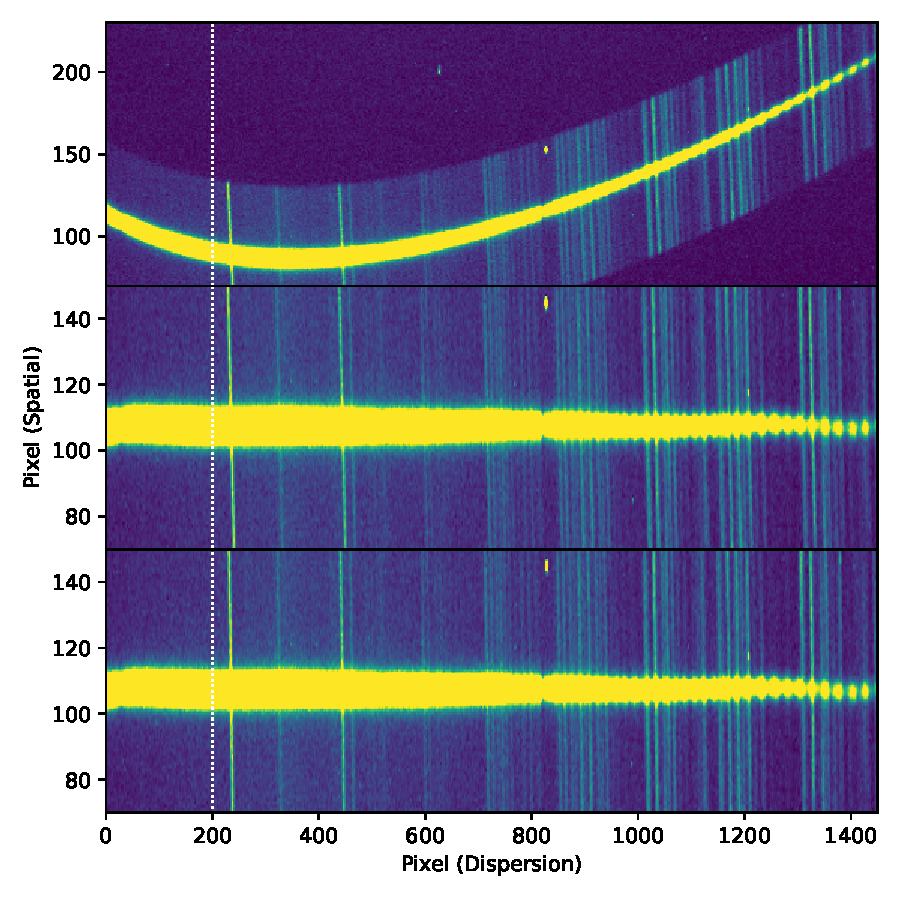
\includegraphics[width=\columnwidth]{fig_02_rectification.pdf}
    \caption{A two-dimensional spectrum from Las Cumbres/FLOYDS is used to demonstrate
    the rectification procedure. The dotted white line is aligned in the
    spatial direction to serve as a visual guide. \textit{Top}: The trimmed image of a
    FLOYDS spectrum. \textit{Middle}: The two-dimensional spectrum is resampled in the
    spatial direction based on the polynomial function of the trace. \textit{Bottom}:
    The two-dimensional spectrum is resampled in the dispersion direction. The
    shifts and scales are found by cross-correlating the sub-spectra divided in
    the spatial direction. This is perpendicular to the tracing process.}
    \label{fig:rectify}
\end{figure}

%%%%%%%%%%%%%%%%%%%%%%%%%%%%%%%%%%%%%%%%%%%%%%%%%%%%%%%%%%%%%%%%%%%%%%%%%%%%%%%%
At the time of writing, this process only works on a single trace. If
more than one trace is found/provided, only the one with the highest prominence
will be processed, where the 
prominence\footnote{\url{https://docs.scipy.org/doc/scipy/reference/generated/scipy.signal.peak_prominences.html}}
is defined as the maximum count of the peak subtracted by the local background. 
The resampling is performed with \texttt{scipy.ndimage.zoom} 
which interpolates with a cubic spline. It is possible to supply a set of
pre-computed polynomials to perform the rectification, which can significantly
speed up the data reduction process of a stable optical system.


%A change in the 
%zeroth order coefficient can shift the bluest part of the spectrum to the
%reddest part, and vice versa. For a stable instrument, this should not affect
%more than a few pixels. However, as long as the effect is identical in the science
%frame and the standard frame they can be calibrated out or trimmed. Furthermore,
%the edges of a detector are usually unusable, so it does not pose any real
%problem.

%%%%%%%%%%%%%%%%%%%%%%%%%%%%%%%%%%%%%%%%%%%%%%%%%%%%%%%%%%%%%%%%%%%%%%%%%%%%%%%%
\subsection{Spectral Extraction}
\label{sec:extract}
There are a few commonly used extraction methods; some work for all kinds of
spectral images, and some only work with specific observing strategies (e.g. the
flat-relative optimal extraction;~\citealt{2014A&A...561A..59Z}). The standard
textbook method is commonly called the \textit{top-hat} extraction or the
\textit{normal} extraction. It simply sums the electron counts over a given size
of the aperture and is robust and easy to use. However, this method does not
deliver the maximal signal-to-noise ratio~(SNR) from the available data. Various
optimal extraction algorithms can maximise the SNR. They work by down-weighting
the wings of the spectral profile where almost all the photons come from the sky
background rather than the source~(see Fig.~\ref{fig:extraction}). The\
improvement is particularly significant for background-limited sources, which
are the case in most observations~(see Fig.~\ref{fig:extraction_compared}).
The extracted spectra and their associated uncertainties and sky background
counts can be plotted for inspection. The residual image can also be exported
for diagnostics.

\begin{figure}
    \centering
    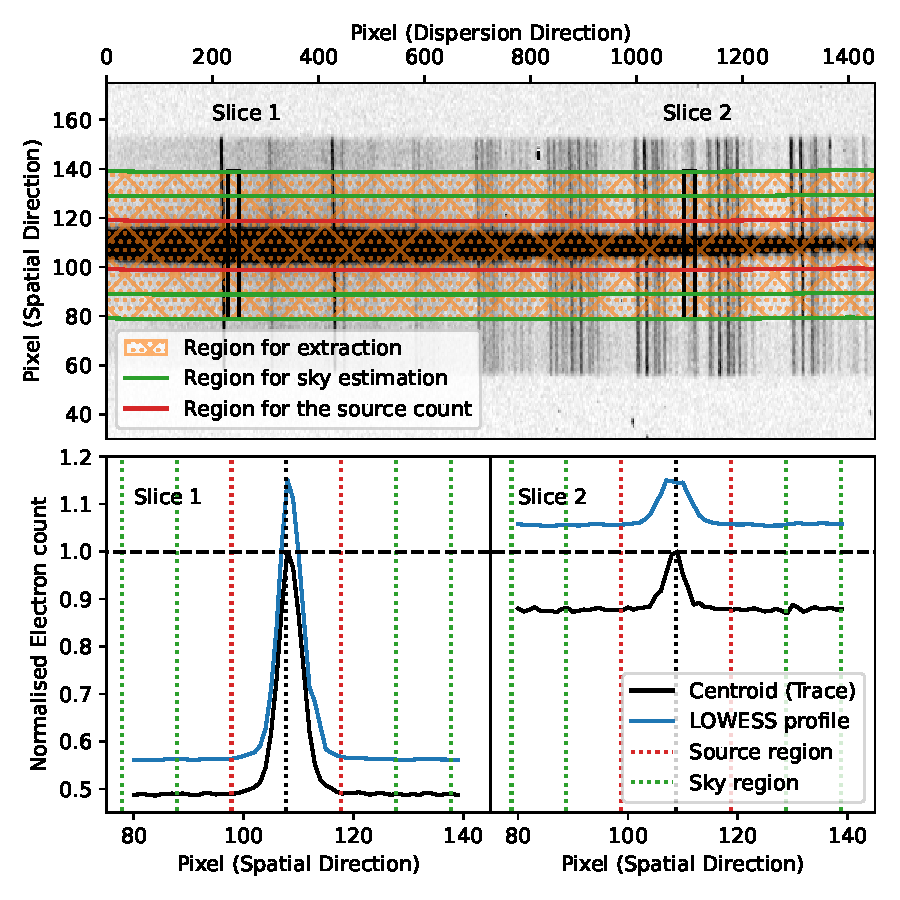
\includegraphics[width=\columnwidth]{fig_03_extraction_profile.pdf}
    \caption{The same spectrum as in Figure~\ref{fig:rectify}. \textit{Top}:
    The regions used for source and sky extractions are marked
    by the red and green boundaries. The light shade of orange
    hash marks the region that is used for spectral extraction.
    The two boxes show the two columns of pixels fitted with
    profiles in the bottom half of the figure (the boxes are inflated
    for clarity). \textit{Bottom}: The independently normalised electron
    counts across the two slices, the much higher baseline on the right indicates a lower signal-to-background ratio. The vertical black dashed
    line is the centroid~(trace) of the spectrum, the two red dashed lines
    mark the regions of the source, and the pairs of green dashed lines on
    each side of the centroid show the regions used for sky extractions,
    respectively. The black line is the measured spectral profile (data), and
    the blue line is the fitted LOWESS line-spread-function (model), offset for
    clarity. The right panel illustrates how an extraction over a non-rectified
    two-dimensional spectrum can lead to an increased sky background level.}
    \label{fig:extraction}
\end{figure}

%%%%%%%%%%%%%%%%%%%%%%%%%%%%%%%%%%%%%%%%%%%%%%%%%%%%%%%%%%%%%%%%%%%%%%%%%%%%%%%%
\subsubsection*{Tophat/Normal Extraction}
\label{sec:tophat}
The top-hat extraction does not weight the pixels for extraction,
so every pixel has an equal contribution to the source count. Thus,
it is very robust in obtaining the total electron count across
a slice of pixels. The sky background count can be extracted
from the regions outside the extraction aperture to be
subtracted from the spectrum.

%%%%%%%%%%%%%%%%%%%%%%%%%%%%%%%%%%%%%%%%%%%%%%%%%%%%%%%%%%%%%%%%%%%%%%%%%%%%%%%%
\subsubsection*{Horne-86 Optimal Extraction}
\citet[hereafter H86]{1986PASP...98..609H} is the golden standard
of optimal extraction of spectra from modern electronic detectors.
We follow the H86 recipe except for the profile modelling,
where we provide three options: The first is a fixed Gaussian
profile, the second uses LOcally Weighted Scatterplot
Smoothing~\citep[LOWESS]{doi:10.1080/01621459.1979.10481038}
regression to fit for a polynomial, and the third accepts
a manually supplied profile.

%%%%%%%%%%%%%%%%%%%%%%%%%%%%%%%%%%%%%%%%%%%%%%%%%%%%%%%%%%%%%%%%%%%%%%%%%%%%%%%%
The default option is to use the Gaussian fit because it is
more robust against noise, cosmic ray contamination and detector
artefacts. It is particularly useful in extracting a faint
spectrum when the image is dominated by background noise as the
Gaussian profile is constructed by fitting the line-spread
function from the total stack of all the
sub-spectra~(as described in Sec.~\ref{sec:tracing}).
LOWESS, on the other hand, would do a better job in fitting
the profile of a resolved galaxy. In any case, the quality
of the extraction from a valid profile should be at least as
good as that performed with the top-hat extraction method.

%%%%%%%%%%%%%%%%%%%%%%%%%%%%%%%%%%%%%%%%%%%%%%%%%%%%%%%%%%%%%%%%%%%%%%%%%%%%%%%%
\subsubsection*{Marsh-89 Optimal Extraction}
\citet[hereafter M89]{1989PASP..101.1032M} extends on the H86 algorithm by
fitting the change in the shape and centroid of the profile from one end of the
spectrum to the other. It is very suited for extracting a highly tilted
spectrum where the tilting direction is aligned with \textbf{one} direction in
the $x$- or the $y$-axis of the detector. The algorithm still relies on the
assumption that the spatial and dispersion directions are orthogonal across
the entire frame (in the detector pixel coordinates). In \textsc{ASPIRED}, we
adapt Prof. Ian Crossfield's set of public \textsc{Python 2} code for
Astronomy\footnote{\url{https://people.ucsc.edu/~ianc/python/}}$^,$\footnote{\url{https://crossfield.ku.edu/python/}}
to \textsc{Python 3}.

\begin{figure}
    \centering
    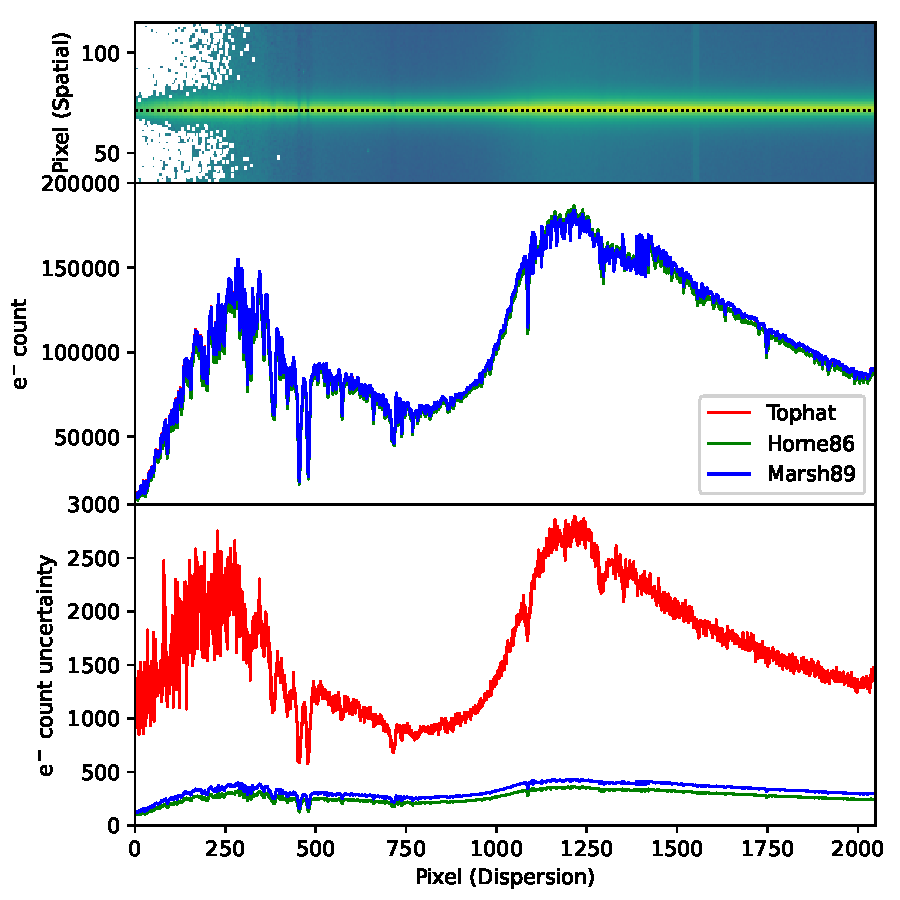
\includegraphics[width=\columnwidth]{fig_04_extraction_compared.pdf}
    \caption{\textit{Top}: the VLT/FORS2 spectrum and the trace of the standard
    star LTT\,7379. \textit{Middle}: The extracted spectra in electron counts
    using the three extraction methods are very similar. \textit{Bottom}: The
    uncertainties with the three extraction methods in units of electron counts.
    The top-hat method is clearly noisier than the two optimal methods.
    \textcolor{red}{Extraction using \texttt{Horne86} and \texttt{Marsh89} algorithm produce
    almost identical outputs.}}
    \label{fig:extraction_compared}
\end{figure}

%%%%%%%%%%%%%%%%%%%%%%%%%%%%%%%%%%%%%%%%%%%%%%%%%%%%%%%%%%%%%%%%%%%%%%%%%%%%%%%%
\subsection{Wavelength Calibration}
As mentioned, the wavelength calibration is powered by \textsc{rascal}, which is
a concurrent development to this work. All the public functions from
\textsc{rascal} are available in \textsc{ASPIRED} so users can have fine control
over the calibration. It works by applying Hough transform to a set of
peak\,(pixel)--line\,(wavelength) pairs (Hough pairs), and then identifying the
most probable set of Hough pairs that can be described by a polynomial
function that satisfies the required residual tolerance limit~(see more
details in \citealt{2020ASPC..527..627V})

The diagnostic plots available are the set provided by \textsc{rascal}.
They include (i)~the spectrum of the arc lamp extracted using the traces from
the science and standard frames, the peak of the arc lines are also marked;
(ii)~the Hough pairs and their constraints in the parameter space;
and (iii)~a plot showing the best fit solution, the residual of the solution,
and the pixel-wavelength relation~(Fig.~\ref{fig:wavecal}).


Alternatively, the polynomial coefficients for the wavelength calibration can be
supplied manually, which would be useful for stable instruments in which the
variations in the dispersion are negligible. All the lines in the
\textcolor{red}{range of } 100 to 30\,000 \AA\ 
available from the search form of the National Institute of Standards and
Technology~(NIST) Physical Measurement Laboratory are included, but we strongly
recommend providing arc lines manually since arc lamps, even of similar type,
vary between manufacturers and the conditions.

\begin{figure}
    \centering
    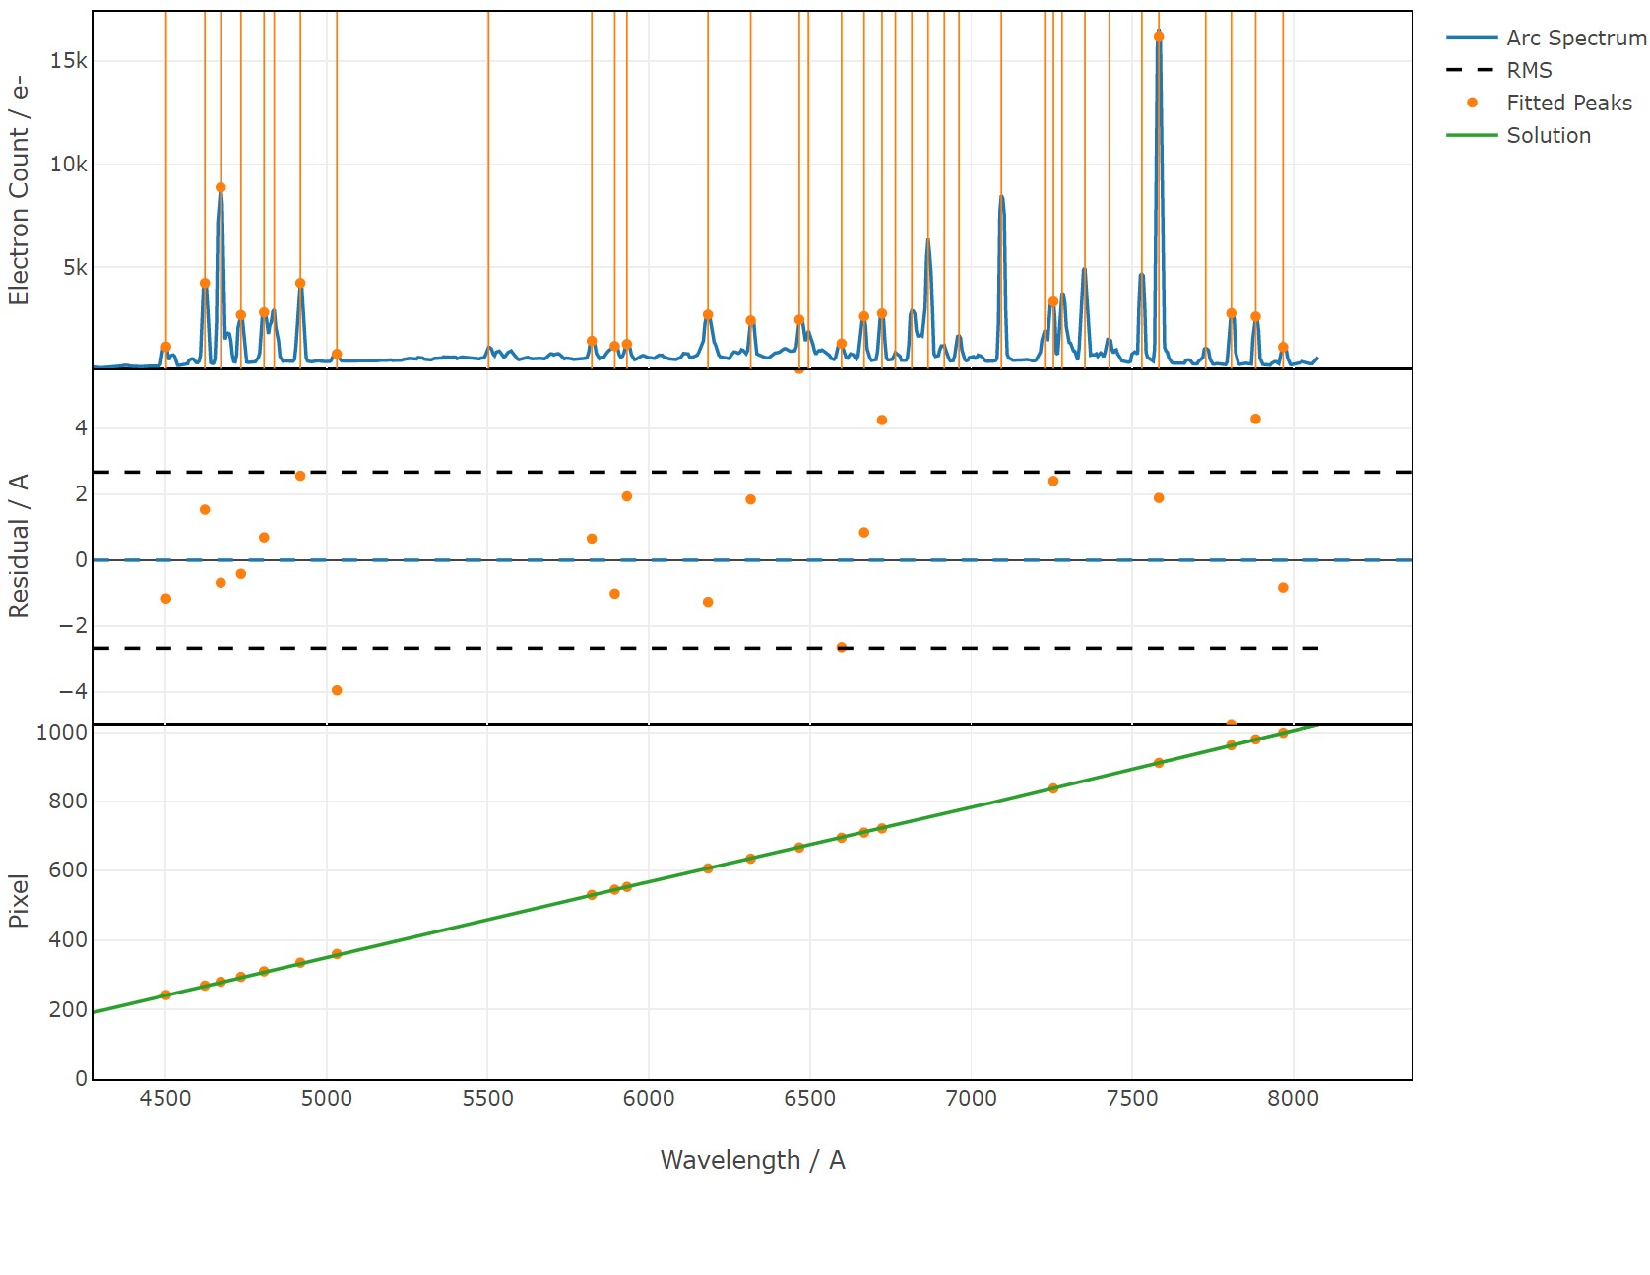
\includegraphics[width=\columnwidth]{fig_05_wavelength_calibration_diagnostics.pdf}
    \caption{The native wavelength calibration diagnostic plots from \textsc{rascal}.
    \textit{Top}: the arc is plotted in blue, the fitted peaks are marked by
    the orange dots. \textit{Middle}: The residual plot shows the difference
    between the fitted peaks and the true wavelengths. \textit{Bottom}: The
    pixel-wavelength function (green) is overplotted with the fitted
    peaks (orange).}
    \label{fig:wavecal}
\end{figure}

%%%%%%%%%%%%%%%%%%%%%%%%%%%%%%%%%%%%%%%%%%%%%%%%%%%%%%%%%%%%%%%%%%%%%%%%%%%%%%%%
\subsection{Flux Calibration}
\textsc{ASPIRED} is designed to address the common case where targets and
reference standards are observed contemporaneously in close succession. It is
well suited to constructing unsupervised, automated pipelines for stable and
repeatable instruments. In such cases, an instrument sensitivity function can be
created from several standard targets, stored and applied to many science target
observations. At the time of writing, \textsc{ASPIRED} cannot construct a
sensitivity function from multiple frames, but it can accept a user-supplied
polynomial function to apply the calibration.
 
The process of deriving a sensitivity function is by comparing a
wavelength-calibrated standard spectrum with the literature values to map the electron count to flux as a function of wavelength. \textcolor{red}{All
the standard stars available in \textsc{iraf}, on the Issac Newton Group of
Telescopes webpage, and on the ESO webpage -- \textit{Optical and UV
Spectrophotometric Standard Stars}} are available on \textsc{ASPIRED}. We
call the set of data a \textit{library}, and provide below the complete
listing of sources and references for each of the libraries where available.

\subsection*{European Southern Observatory~(ESO)}
The ESO standard spectra are grouped into five sets, they can be downloaded from \url{https://www.eso.org/sci/observing/tools/standards/spectra/}:

\begin{itemize}
    \item \texttt{esoctiostan} -- CTIO standards from \citet{1992PASP..104..533H, 1994PASP..106..566H}
    \item \texttt{esohststan} -- \textit{HST} standards from \citet{1995AJ....110.1316B, 1996AJ....111.1743B}
    \item \texttt{esookestan} -- Oke standards from \citet{1990AJ.....99.1621O}
    \item \texttt{esowdstan} -- White dwarf standards from \citet{1995AJ....110.1316B}
    \item \texttt{esoxshooter} -- ESO \textit{VLT} X-shooter standards from \citet{2014Msngr.158...16M, 2014A&A...568A...9M}
\end{itemize}


\subsection*{Issac Newton Group of Telescopes~(ING)}

The ING listing is grouped into five sets by the last name of the authors\footnote{\url{http://www.ing.iac.es/Astronomy/observing/manuals/html_manuals/tech_notes/tn065-100/workflux.html}}.

\begin{itemize}
    \item \texttt{ing\_oke} -- \citet{1990AJ.....99.1621O} standards
    \item \texttt{ing\_sto} -- \citet{1977ApJ...218..767S} standards
    \item \texttt{ing\_og} -- \citet{1983ApJ...266..713O} standards
    \item \texttt{ing\_mas} -- \citet{1988ApJ...328..315M} standards
    \item \texttt{ing\_fg} -- \citet{1984PASP...96..530F} standards
\end{itemize}

\subsection*{\texttt{iraf} Standards}
The complete listing of \texttt{iraf} standards can be found at
\url{https://github.com/iraf-community/iraf/tree/main/noao/lib/onedstds}.
References are included where they are available.

\begin{itemize}
    \item \texttt{irafblackbody}
    \item \texttt{irafbstdscal} -- KPNO IRS standards (i.e.\ those from the Henry Draper~(HD) catalogue)
    \item \texttt{irafctiocal} -- The original CTIO standards \citet{1983MNRAS.204..347S, 1984MNRAS.206..241B}
    \item \texttt{irafctionewcal} -- The updated CTIO standards \citet{1992PASP..104..533H, 1994PASP..106..566H}
    \item \texttt{irafiidscal} -- KPNO IIDS standards \citet{1988ApJ...328..315M}
    \item \texttt{irafirscal} -- KPNO IRS standards \citet{1988ApJ...328..315M}
    \item \texttt{irafoke1990} -- \textit{HST} standards \citet{1990AJ.....99.1621O}
    \item \texttt{irafredcal} -- KPNO IRS standards \& IIDS \citet{1988ApJ...328..315M} with wavelength beyond 8\,370\,$\mathrm{\AA}$
    \item \texttt{irafspechayescal} -- KPNO standards \citet{1988ApJ...328..315M}
    \item \texttt{irafspec16cal} -- CTIO standards \citet{1992PASP..104..533H, 1994PASP..106..566H} at 16$\mathrm{\AA}$ interval
    \item \texttt{irafspec50cal} -- KPNO standards \citet{1988ApJ...328..315M, 1990ApJ...358..344M} at 50$\mathrm{\AA}$ interval
\end{itemize}



The calibration can be done in either AB magnitude or
flux density~(per unit wavelength). The two should give similar
results, but the response functions found would not be equivalent
because fitting to magnitudes is in logarithmic space and smoothing~(see
below) will have a different effect compared to flux fitting.

%%%%%%%%%%%%%%%%%%%%%%%%%%%%%%%%%%%%%%%%%%%%%%%%%%%%%%%%%%%%%%%%%%%%%%%%%%%%%%%%
\subsubsection*{Smoothing}
A Savitzky-Golay smoothing
filter\footnote{\url{https://docs.scipy.org/doc/scipy/reference/generated/scipy.signal.savgol_filter.html}}~\citep[hereafter, SG-filter]{1964AnaCh..36.1627S}
can be applied to the data before computing the sensitivity curve. This function
works by fitting low-order polynomials to localised subsets of the data to
suppress noise in the data at each point interval. It is similar to the
commonly used median boxcar filter but uses more weighted information to
retain information better while removing noise. This can be used independently
or with continuum fitting (see below), which uses a LOWESS filter. By default,
the smoothing is turned off and when it is used, it is defaulted to
remove only significant noise~(e.g.\ from unsubtracted cosmic rays).

%%%%%%%%%%%%%%%%%%%%%%%%%%%%%%%%%%%%%%%%%%%%%%%%%%%%%%%%%%%%%%%%%%%%%%%%%%%%%%%%
\subsubsection*{Continuum Fitting}
\textcolor{red}{It is optional for the sensitivity function to be} derived from
the continuum of the standard spectrum. This \textcolor{red}{removes} absorption
lines in the standard spectrum. This process is strongly dependent on both the
resolution of the literature and the observed standards, as well as the
absorption lines present in them. 
The continuum is \textcolor{red}{found using the \textsc{specutils}'s
\texttt{fits\_continuum}}. This can remove any outlying random noise and
absorption lines when computing the  sensitivity. Users are reminded to be
cautious with this procedure as removing the absorption features in computing
the sensitivity function can significantly affect the flux calibration near
the absorption features.

%%%%%%%%%%%%%%%%%%%%%%%%%%%%%%%%%%%%%%%%%%%%%%%%%%%%%%%%%%%%%%%%%%%%%%%%%%%%%%%%
\subsubsection*{Sensitivity Function}
The sensitivity function is computed by dividing the observed standard spectrum
by the literature one and then interpolating the result using a spline or a
polynomial function~(Fig.~\ref{fig:fluxcal}). This can be done with or without
any pre-smoothing and/or continuum fitting. In case of a high-resolution
literature standard spectrum~(e.g.\ the ESO X-Shooter standards), the
absorption line profiles should be used as part of the sensitivity computation.
While in the case of the standard stars from \citet{1990AJ.....99.1621O},
which removed absorption lines when producing the standard spectra, a
smooth continuum of the observed spectrum should be used for computing
the sensitivity function. Users can also manually supply a sensitivity function
as a callable function that accepts a wavelength value and returns the $\log$
of the sensitivity value at that wavelength. When such a function is provided
manually, it is assumed to be in the unit of flux per second.

\begin{figure}
    \centering
    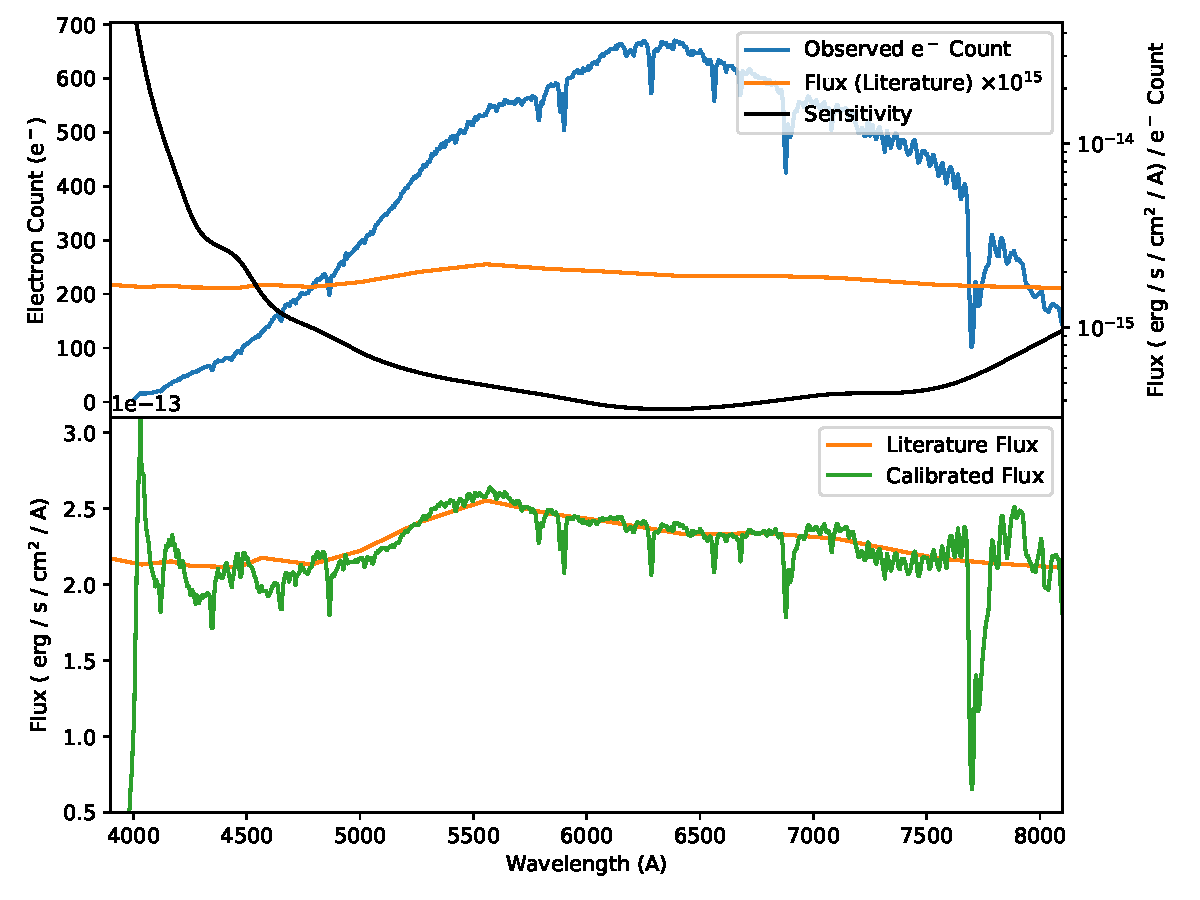
\includegraphics[width=\columnwidth]{fig_06_flux_calibration_diagnostics.pdf}
    \caption{\textit{Top}: The extracted standard spectrum in electron
    counts~(blue), the literature spectrum in units of flux density~(orange),
    and the sensitivity function~(y-axis on the right; black). \textit{Bottom}:
    The literature spectrum (same as the one above) is plotted in orange, and
    the calibrated observed spectrum is plotted in green.}
    \label{fig:fluxcal}
\end{figure}

%%%%%%%%%%%%%%%%%%%%%%%%%%%%%%%%%%%%%%%%%%%%%%%%%%%%%%%%%%%%%%%%%%%%%%%%%%%%%%%%
\subsection{Atmospheric Extinction Correction}
\textsc{ASPIRED} currently has four built-in atmospheric extinction curves (Fig.~\ref{fig:extinction}):

\begin{enumerate}
    \item Roque de los Muchachos Observatory, Spain~(La Palma, 2\,420\,m)\footnote{\url{http://www.ing.iac.es/astronomy/observing/manuals/ps/tech\_notes/tn031.pdf}}
    \item Mauna Kea Observatories, US~\citep[Big Island, Hawaii, 4\,205\,m;][]{2013A&A...549A...8B}
    \item Cerro Paranal Observatory, Chile~\citep[Atacama Desert, 2\,635\,m;][]{2011A&A...527A..91P}
    \item La Silla Observatory, Chile~(Atacama Desert, 2\,400\,m)\footnote{\url{https://www.eso.org/public/archives/techdocs/pdf/report\_0003.pdf}}
\end{enumerate}

These curves describe the extinction in magnitude per airmass as a function of wavelength,
roughly between $3\,000$ and $10\,000$\,\AA. Alternatively, a callable function
in the appropriate units can be supplied to perform the extinction correction.
The airmass of the observation can be found from the header if it is reported
using the conventional keywords for airmass.
\begin{figure}
    \centering
    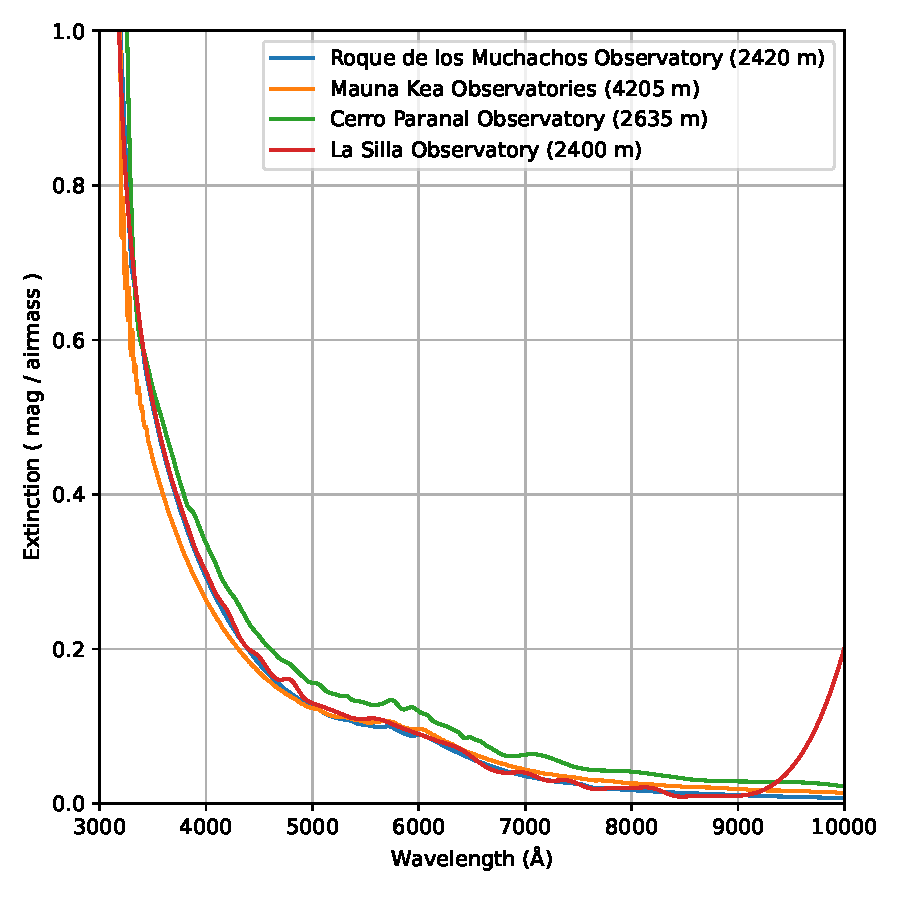
\includegraphics[width=\columnwidth]{fig_07_extinction_curves.pdf}
    \caption{Extinction curves measured at Roque de los
    Muchachos Observatory~(2420\,m; blue), Mauna Kea Observatories~(4\,205\,m;
    orange), Cerro Paranal Observatory~(2\,635\,m; green), and La Silla
    Observatory~(2400\,m; red). The extinction table of La Silla Observatory
    terminates at $9\,000$\,\AA. The rise at the red end of the curve is an
    undesired artefact due to extrapolation using a cubic spline (included in the original data). We are
    explicitly plotting this range to serve as a warning since we opt to
    preserve the raw data as provided without appending fake data points.}
    \label{fig:extinction}
\end{figure}

%%%%%%%%%%%%%%%%%%%%%%%%%%%%%%%%%%%%%%%%%%%%%%%%%%%%%%%%%%%%%%%%%%%%%%%%%%%%%%%%
\subsection{Telluric Absorption Removal}
During the process of generating the sensitivity function, masks are used
over the telluric regions to generate the telluric absorption
profile from the standard star. The default masking regions are $6\,850-6\,960$
and $7\,580-7\,700$\ \AA\ only. This telluric profile can then be multiplied
by a factor to be determined in order to remove the telluric absorption
features in the science target. The best multiplicative factor is found
by minimising the difference between the continuum and the telluric-absorption
corrected spectrum simultaneously for both the sampled telluric regions~(there are only two ranges in the default setting, but if more regions are
provided, this process will apply to all of them simultaneously).
An \textbf{extra} multiplier can be manually provided to adjust the
strength of the subtraction. This is designed for manually fine-tuning the
absorption factor; otherwise, it defaults to $1.0$.

%%%%%%%%%%%%%%%%%%%%%%%%%%%%%%%%%%%%%%%%%%%%%%%%%%%%%%%%%%%%%%%%%%%%%%%%%%%%%%%%
\subsection{Resampling}
All the operations above are performed as a function of the native detector
pixels. This includes the telluric absorption corrections as the telluric profile
is generated in the standard spectrum pixel/wavelength coordinates. The
correction applied to the target spectrum is performed using an interpolated
function of the profile at the wavelengths of the target spectrum. 

Many legacy
software packages can only read the spectrum using the header information to create
the wavelength coordinates using only three parameters: the wavelength of the
first element of the spectral array, the bin width of each wavelength
coordinate, and the length of the spectral array. This requires a uniformly
sampled wavelength axis, which never happens naturally as there is always some
level of image distortion at the detector plane. A resampling is necessary
to turn the data into such a format.

The resampling is performed with the \textsc{spectres} package. Although
this package allows non-uniform wavelength spacing resampling, we are only
using it for uniform resampling for the purpose of exporting the data as FITS
files.

%%%%%%%%%%%%%%%%%%%%%%%%%%%%%%%%%%%%%%%%%%%%%%%%%%%%%%%%%%%%%%%%%%%%%%%%%%%%%%%%
\subsection{Output}
At the time of writing, 22 types of output to CSV and FITS files are supported.
Each CSV has the various exported data (see below) stored in a separate columns, while the FITS has
the data stored in a separate Header Data Units (HDUs). Each spectrum is exported
as a separate file. At the time of writing, the header is not exported when the
output option is CSV. The options for output are:

\begin{enumerate}
    \item \texttt{trace} -- two columns/HDUs containing the pixel coordinates
    of the trace and its width in the spatial direction.
    \item \texttt{count} -- three columns/HDUs containing the electron count
    of the spectrum, its uncertainty, and the sky background.
    \item \texttt{weight\_map} -- one column/HDU for the extraction profile,
    in top hat and \texttt{horne86} extraction this is a one dimensional array,
    while the \texttt{marsh90} extraction returns a two dimensional array.
    \item \texttt{arc\_spec} -- three columns/HDUs for the one-dimensional arc
    spectrum, pixel coordinates of the arc line position (sub-pixel precision),
    and the pixel coordinates of the arc line effective position~(e.g.\ accounting for chip gaps) in the dispersion direction.
    \item \texttt{wavecal} -- one column/HDU for the polynomial coefficients
    for wavelength calibration. The header contains the information regarding the
    polynomial type.
    \item \texttt{wavelength} -- one column/HDU for the wavelength at the
    native pixel position.
    \item \texttt{sensitivity} -- one column/HDU containing the sensitivity
    function of the detector as a function of the native detector pixel.
    \item \texttt{flux} -- three columns/HDUs containing the
    flux of the spectrum, its uncertainty, and the sky background.
    \item \texttt{atm\_ext} -- one column/HDU containing the atmospheric
    extinction correction factor at each wavelength position.
    \item \texttt{flux\_atm\_ext\_corrected} -- three columns/HDUs containing
    the atmospheric extinction corrected flux of the spectrum, its
    uncertainty, and the sky background.
    \item \texttt{telluric\_profile} -- one column/HDU containing the telluric
    absorption profile from the standard spectrum.
    \item \texttt{flux\_telluric\_corrected} -- three columns/HDUs containing
    the telluric absorption corrected flux, uncertainty, and the sky
    background.
    \item \texttt{flux\_atm\_ext\_telluric\_corrected} -- three columns/HDUs
    containing the atmospheric extinction and telluric corrected flux,
    uncertainty, and the sky background.
    \item \texttt{wavelength\_resampled} -- one column/HDU containing the
    wavelength at each resampled position.
    \item \texttt{count\_resampled} -- three columns/HDUs containing the
    electron count of the spectrum, its uncertainty, and the sky background
    being subtracted during the extraction process at the resampled wavelength.
    \item \texttt{sensitivity\_resampled} -- one column/HDU containing the
    sensitivity function of the detector as a function of resampled wavelength.
    \item \texttt{flux\_resampled} -- three columns/HDUs containing the
    flux of the spectrum, its uncertainty, and the sky background at the
    resampled wavelength.
    \item \texttt{atm\_ext\_resampled} -- one column/HDU containing the
    atmospheric extinction correction factor at the resampled wavelength.
    \item \texttt{flux\_resampled\_atm\_ext\_corrected} -- three columns/HDUs
    containing the atmospheric extinction corrected flux of the spectrum, its
    uncertainty, and the sky background at the resampled wavelength.
    \item \texttt{telluric\_profile\_resampled} -- one column/HDU containing
    the telluric absorption profile from the standard spectrum at the resampled
    wavelength.
    \item \texttt{flux\_resampled\_telluric\_corrected} -- three columns/HDUs
    containing the telluric absorption corrected flux, uncertainty, and the sky
    background at the resampled wavelength.
    \item \texttt{flux\_resampled\_atm\_ext\_telluric\_corrected} -- three
    columns/HDUs containing the atmospheric extinction and telluric absorption
    corrected flux, uncertainty, and the sky background at the resampled
    wavelength.
\end{enumerate}


%%%%%%%%%%%%%%%%%%%%%%%%%%%%%%%%%%%%%%%%%%%%%%%%%%%%%%%%%%%%%%%%%%%%%%%%%%%%%%%%
\textcolor{red}{\section{Validation}
\label{sec:examples}
}
Being a flexible toolkit, \textsc{ASPIRED} is not designed to reduce data for a
specific instrument. Instead, it can be customised to suit many configurations,
as long as they are long-slit-like. We demonstrate this here with data products
from eight different instruments, most of which have conventional long-slit
settings. A summary of the following example reductions is tabulated in
Table~\ref{tab:summary}.

\textcolor{red}{The purpose of the comparison made here is to demonstrate that
the reductions are sufficiently consistent with some spectra in the literature
for a range of instruments and astrophysical sources. However, a full
systematic comparison is beyond the scope of this work. Such a level of
detailed validation would be the most useful if any service providers wish to
adopt \textsc{ASPIRED} as the official reduction tool, and that shall be
included in future work.}

\textcolor{red}{\subsection{Repeatability}}
\textcolor{red}{In order to demonstrate the reproducibility and repeatability,
we opt to calibrate the standard star BD\,33+2642 against Hiltner\,102 on
eight nights that \textit{LT}/SPRAT collected both on the same night during
semester 2022\,B. We require the transparency to be photometric and the seeing
is better than 2'' as reported by the autoguider. Because of the robotic
observing nature of the LT, standard stars are only taken in the beginning
and at the end of the nights. The data used are not taken immediately
before or after each other, the weather effect cannot be calibrated out,
we only attempt to apply atmospheric extinction corrections and telluric
absorption corrections. From the reprocessing, We find a typical spread in
the residual of roughly 1-2\%. The absolute deviation is within 3\% apart from
around the Telluric absorption regions and at the H$\gamma$ line at 4340\,\AA\
that are observed at low detector efficiency~(see Fig.~\ref{fig:repeatability}).}

\begin{figure}
    \centering
    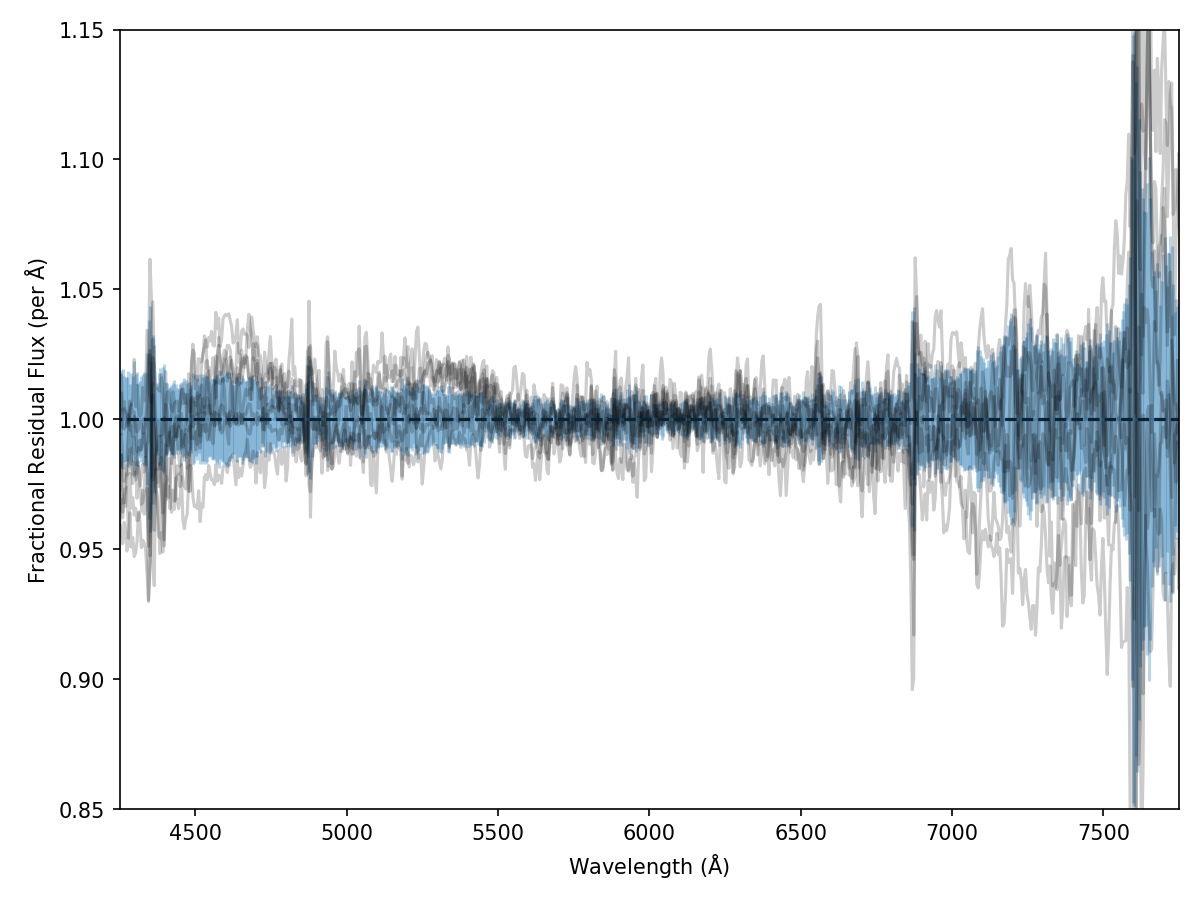
\includegraphics[width=\columnwidth]{fig_08_sprat_standards_compared.png}
    \caption{\textcolor{red}{Fractional residual in the calibrated flux of BD\,33+2642 using
    Hiltner\,102 as a standard star taken with \textit{LT}/SPRAT. Each grey
    lines show the residual between the median spectrum of the eight spectra
    taken on different nights. The blue area shows the 1 standard deviation
    of the scatter in the residual. The spikes above 5\% residual are the
    H$\gamma$ at 4340\,\AA\ and the oxygen telluric features at the 6869 and
    7605\,\AA\ . The residuals that are larger on the two ends are expected as
    the signal-to-noise ratios drop with the detector efficiency on either
    side.}}
    \label{fig:repeatability}
\end{figure}

\textcolor{red}{\subsection{Example Data Reduction Results}
}
In the case of Gemini/GMOS, a single spectrum is exposed onto
three detectors, and each detector is read out with four amplifiers. The bias 
subtraction is also unconventional, so all the image data reduction procedures
have to be done outside of \textsc{ASPIRED} beforehand. We compare our reduction against
the official one for the kilonova AT 2017gfo\footnote{\url{https://www.wiserep.org/}}~\citep{2017ApJ...848L..32M}. 

Las Cumbres Observatory/FLOYDS has a beam-splitter to expose the first-order
red beam and the second-order blue beam into two non-parallel
curved spectra on a single chip. Both the northern and southern FLOYDS suffers
from strong fringing effects. This is not handled natively through the API of 
\textsc{ASPIRED}. Instead, the correction was done by directly modifying the
electron \texttt{count} of the \texttt{OneDSpec} object. The fringe subtraction
workflow follows that of the official
pipeline\footnote{\url{https://github.com/LCOGT/floyds_pipeline}}. Here, the
Type II supernova iPTF14hls is used as an example for
comparison~\citep{2017Natur.551..210A}.

\textit{LT}/SPRAT is a high throughput low-resolution spectrograph with
a conventional optical design; in this case, we compare our reduction to that published for a nova 
shell DO Aql from a stack of four individual 
exposures\footnote{\url{https://telescope.livjm.ac.uk/cgi-bin/lt_search}}~\citep{2020MNRAS.499.2959H}. 

The \textit{VLT}/FORS2 data
of the helium accretor~(AM CVn) V418 Ser stacked from 21 individual exposures is
used as our last comparison~\citep{2020MNRAS.496.1243G}. 

The first three spectra were 
compared against data reduction from \textsc{iraf}-based pipelines, while the
last one is reduced with \textsc{Molly}\footnote{
\url{https://cygnus.astro.warwick.ac.uk/phsaap/software/molly/html/INDEX.html}}~\citep{2019ascl.soft07012M},
which is built on top of \textsc{STARLINK}. All of our reductions are resampled to match
the resolution in the equivalent published spectra. Our comparisons are shown in Figure \ref{fig:reduction_compared}.

%%%%%%%%%%%%%%%%%%%%%%%%%%%%%%%%%%%%%%%%%%%%%%%%%%%%%%%%%%%%%%%%%%%%%%%%%%%%%%%%
Aside from the comparison against the independently and externally calibrated
spectra above, we also illustrate a few cases of extractions concerning
other use cases that \textsc{ASPIRED} is capable of dealing with. In the top set
of spectra in Figure~\ref{fig:use_cases}, the \textit{GTC}/OSIRIS data show a
blue large amplitude pulsator with many resolved absorption lines in both the
science and the standard targets~(Feige 110\footnote{
\url{https://www.eso.org/sci/observing/tools/standards/spectra/feige110.html}};
~\citealp{2022MNRAS.511.4971M}). With a poorly computed sensitivity curve, we
expect many small bump features in the the spectra and their continuum would
not agree in the overlapping wavelength range as polynomials tend to run away
at the edges of the fitted range of the wavelength solution. In the middle,
the \textit{TNG}/DOLORES case shows a simultaneous tracing of a common proper
motion system (three bodies resolved as two components) containing an M dwarf
and a pair of eclipsing M dwarf--white dwarf binary~\citep{2022MNRAS.509.4171K},
separated by 5'' incidented on the same long-slit in a single exposure.
At the bottom is a set of three spectra taken with \textit{WHT}/ISIS and ACAM.
It demonstrates the reduction of a set of data with extremely low signal-to-noise
for an ultra-cool white dwarf with a smooth blackbody-like
spectrum~\citep{2020MNRAS.493.6001L}. The tracing and extraction are only
possible after careful cosmic ray removal and trimming of the images. The
spectral shape of the ISIS spectra in both the blue and the red arms are in good
agreement with the ACAM spectrum. And these independently flux calibrated
spectra agree well with each other in the overlapping wavelength ranges.

%%%%%%%%%%%%%%%%%%%%%%%%%%%%%%%%%%%%%%%%%%%%%%%%%%%%%%%%%%%%%%%%%%%%%%%%%%%%%%%%
To summarize, our test cases cover the most commonly encountered possible
problematic data (red or blue dominated spectra, narrow/broad
absorption/emission lines, featureless spectra, closely spaced (resolved)
line spectra and curved spectra) and demonstrate that \textsc{ASPIRED} can
produce spectral products at a quality comparable to \textcolor{red}{some
selected published spectra}.

%%%%%%%%%%%%%%%%%%%%%%%%%%%%%%%%%%%%%%%%%%%%%%%%%%%%%%%%%%%%%%%%%%%%%%%%%%%%%%%%
\begin{table*}
    \begin{tabular}{l|c|c|c}\hline
        Telescope/Instrument & Object Type                                 & Grating             & Arc \\\hline\hline
        \multicolumn{4}{c}{Conventional Long-slit Setup}\\\hline

        \textit{GTC}/OSIRIS           & BLAP (ZGP-BLAP-09)                          & R2500U \& R1000B    & HgArNe \\
        \textit{LT}/SPRAT      & Nova shell remnant (DO Aql)                 & 600\,l/mm           & Xe \\
        \multirow{2}{*}{\textit{TNG}/DOLORES}          & Common Proper Motion \& Eclipsing System     & \multirow{2}{*}{LR-B}                & \multirow{2}{*}{ArKrNeHg} \\
                             & (ZTF J192014.13+272218.1)     &           &  \\
        \textit{VLT}/FORS             & AM CVn (V418 Ser)                           & 600B                & HeHgCd \\
        \textit{WHT}/ACAM             & Ultracool White Dwarf (PSO J180153.69+625420.24)       & V400                & CuAr \\
        \textit{WHT}/ISIS             & Ultracool White Dwarf (PSO J180153.69+625420.24)       & R300B \& R300R      & CuAr \\\hline
        \multicolumn{4}{c}{Other Setup}\\\hline
        Las Cumbres/FLOYDS           & Type II-P (iPTF14hls)                       & 235\,l/mm           & HgArZn \\
        Gemini/GMOS          & kilonova (AT 2017gfo)                       & R400 \& B600        & CuAr \\\hline
\end{tabular}
    \caption{List of the eight targets used in Figures~\ref{fig:reduction_compared} \& \ref{fig:use_cases} \textcolor{red}{in alphabetical order of the telescope names}. See body text for references.}
    \label{tab:summary}
\end{table*}

%%%%%%%%%%%%%%%%%%%%%%%%%%%%%%%%%%%%%%%%%%%%%%%%%%%%%%%%%%%%%%%%%%%%%%%%%%%%%%%%
\begin{figure*}
    \centering
    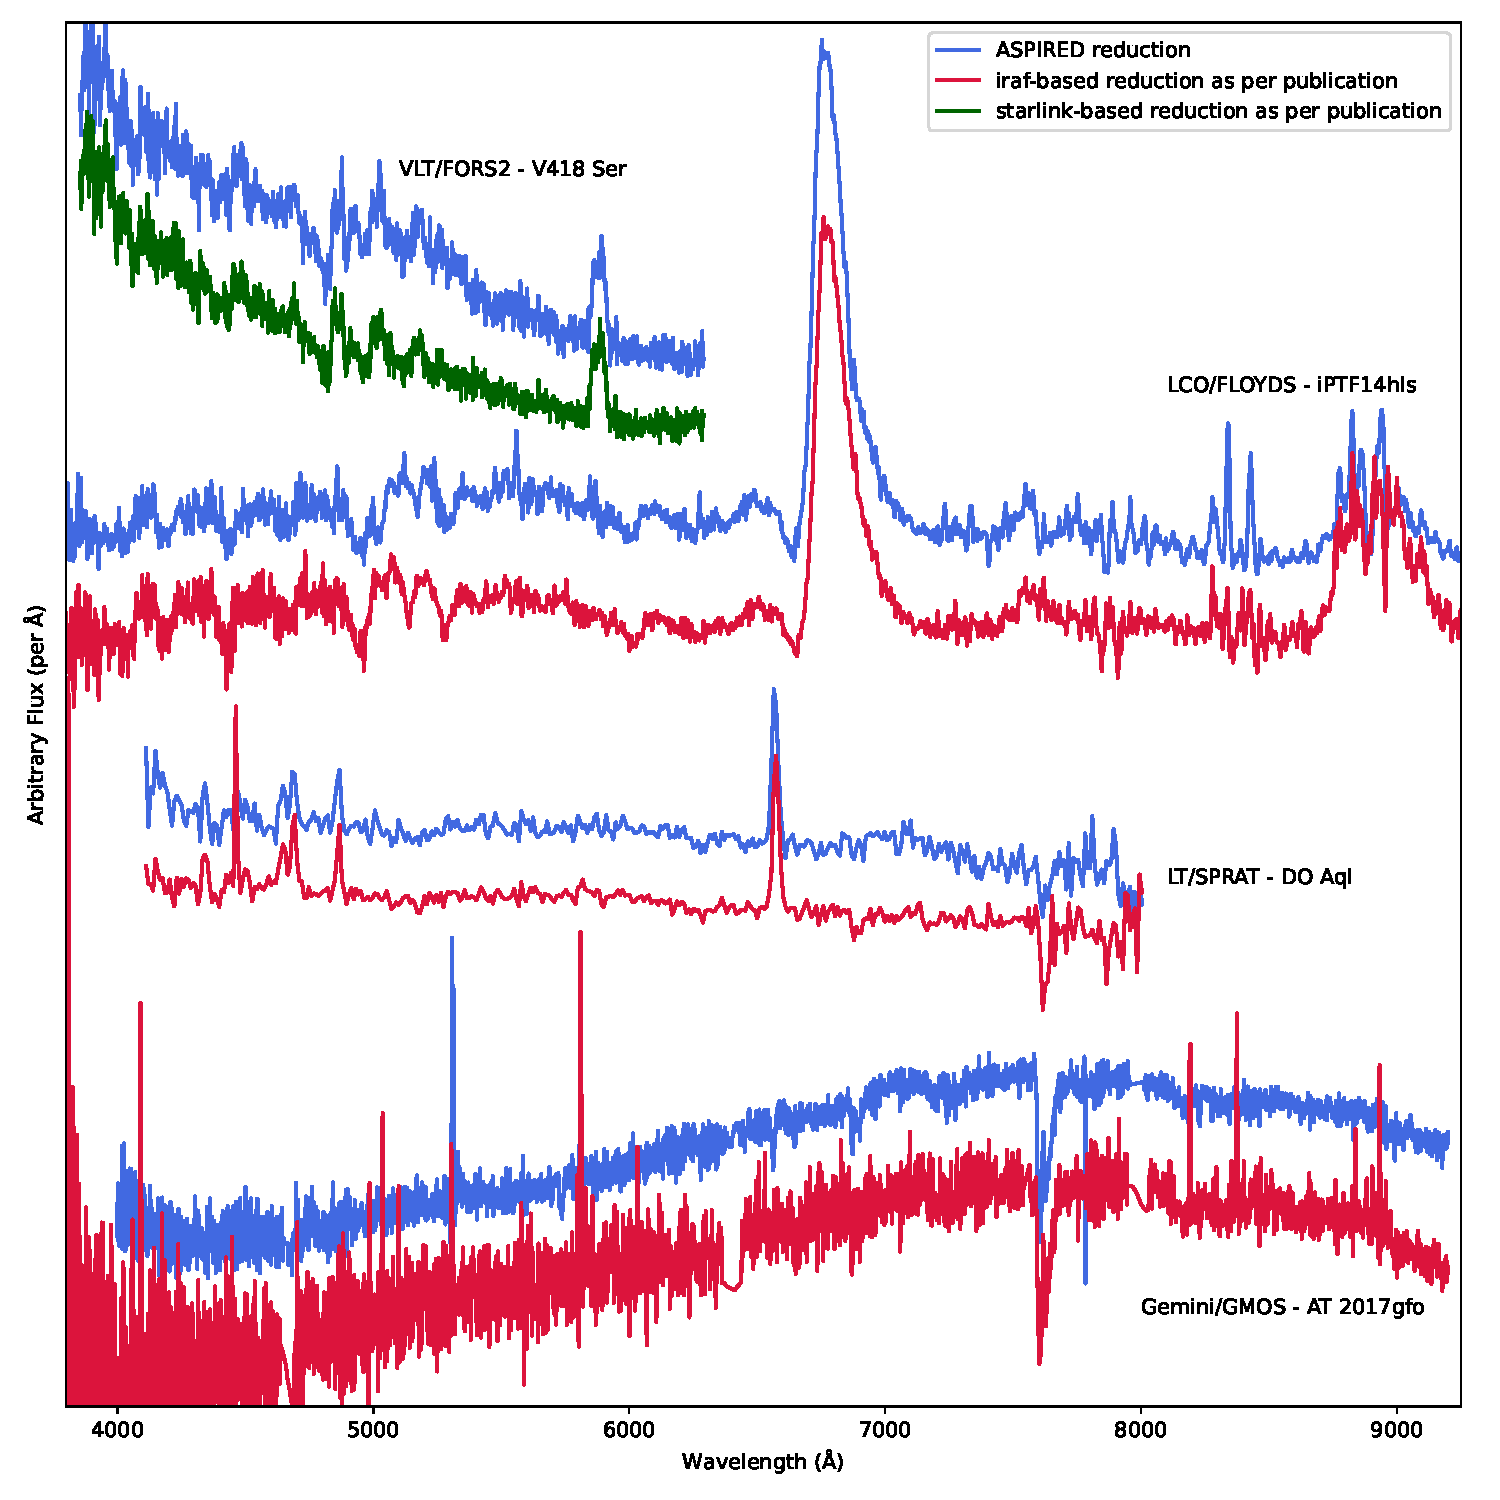
\includegraphics[width=\textwidth]{fig_09_reduction_compared.pdf}
    \caption{From top to bottom are the comparison spectra taken with \textit{VLT}/FORS2,
    Las Cumbres/FLOYDS, \textit{LT}/SPRAT and Gemini/GMOS in long-slit mode. The published FORS2
    spectrum was reduced using \textsc{Molly}~(green) powered by the \textsc{STARLINK}
    library. The other three (red) were reduced using the respective \textsc{iraf}-based
    pipelines. All spectra reduced with \textsc{ASPIRED}~(blue) are optimally extracted using the \cite{1986PASP...98..609H} algorithm and resampled to match
    the respective published spectra. Telluric correction is applied using the default
    setting.}
    \label{fig:reduction_compared}
\end{figure*}

\begin{figure}
    \centering
    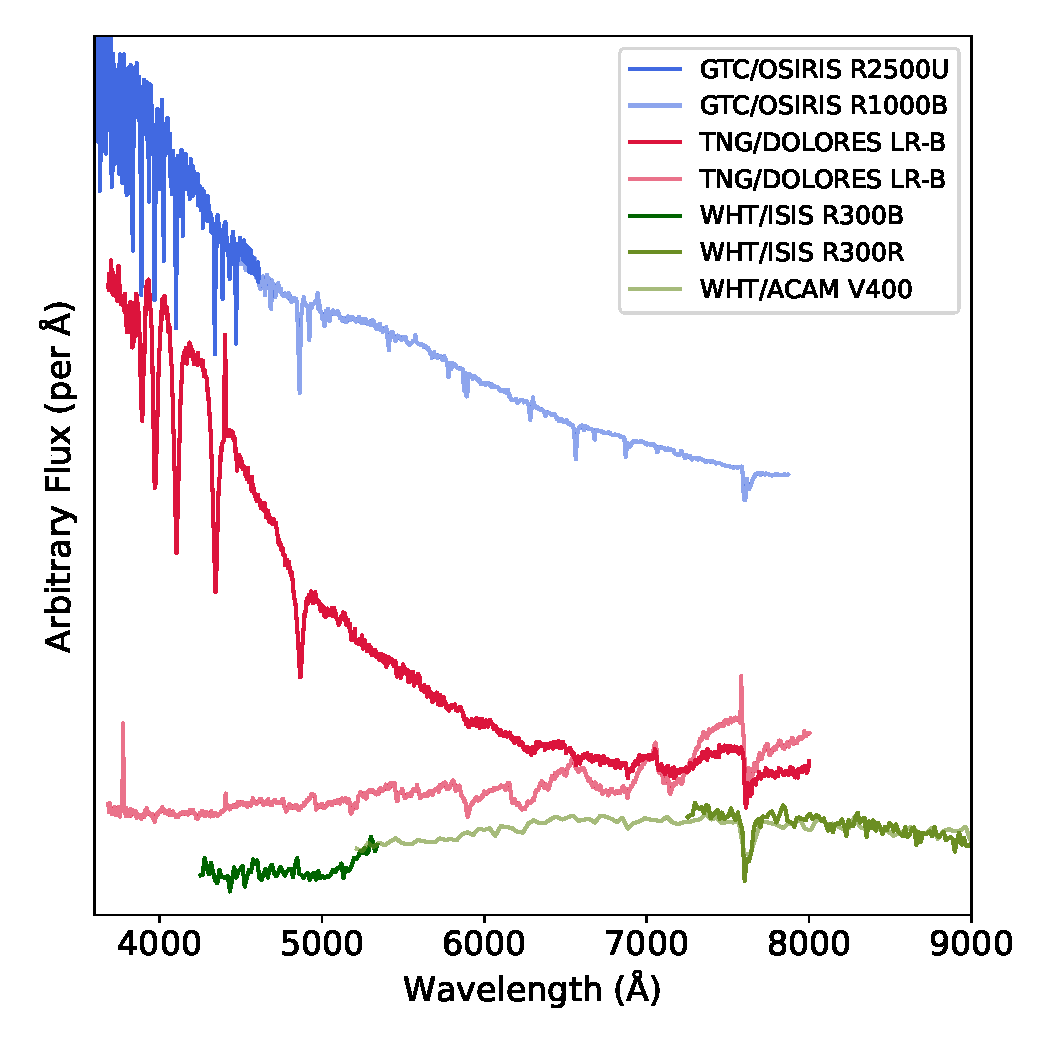
\includegraphics[width=\columnwidth]{fig_10_use_case_plots.pdf}
    \caption{Example extractions of some special cases. Each set of spectra
    uses the same normalisation. All spectra are optimally extracted using the
    \citet{1986PASP...98..609H} algorithm. The \textit{GTC}/OSIRIS (top set in blue hue)
    spectra were flux calibrated in the shorter wavelengths where there are a
    lot of absorption features. With a bad sensitivity curve, we expect many
    small bump features in the the spectra and their continuum would not agree
    in the overlapping wavelength range as polynomials tend to run away at the
    edges. The \textit{TNG}/DOLORES (middle set in red hue) spectra were of two targets where
    the tracing was done simultaneously and then the extraction done
    sequentially. The \textit{WHT}/ISIS and ACAM (bottom set in green hue) data demonstrate
    extracting a target with a very low signal-to-noise ratio. The independently
    flux calibrated spectra agree well with each other in the overlapping
    wavelength ranges.}
    \label{fig:use_cases}
\end{figure}

%%%%%%%%%%%%%%%%%%%%%%%%%%%%%%%%%%%%%%%%%%%%%%%%%%%%%%%%%%%%%%%%%%%%%%%%%%%%%%%%
\section{Distribution}
\label{sec:distribution}

\textsc{ASPIRED} is released under the BSD~(3-Clause) License. The source code
is hosted on \textsc{Github}. The DOI of each version can be found on 
\textsc{zenodo}: \url{https://zenodo.org/record/4127294}. For more
straightforward installation, \textsc{ASPIRED} is also available with the
\textsc{Python Package Index}~(\textsc{PyPI}) so users can install the software with a single command. 
\begin{verbatim}
>> pip install aspired
\end{verbatim}
The latest stable version can be installed with
\begin{verbatim}
>> pip install git+https://github.com/
    cylammarco/ASPIRED@main
\end{verbatim}
and the development version can be installed with 
\begin{verbatim}
>> pip install git+https://github.com/
    cylammarco/ASPIRED@dev-v[Major].[Minor].X
\end{verbatim} where \verb+[Major]+ and \verb+[Minor]+ are the major and minor
version numbers. \verb+X+ is an actual character of the branch name as we only
use separate maintenance branches at the level of minor version granularity.

It is also possible to clone the entire repository
and install with the setup script using
\begin{verbatim}
>> git clone [url to main/dev/a specific commit]
>> python setup.py
\end{verbatim}
ASPIRED is distributed through \textsc{conda} starting from \texttt{v0.4.9}.

\textcolor{red}{
All the reduction scripts for the spectra used in this article can be found at
\url{https://github.com/cylammarco/ASPIRED-apj-article}.} There are also example
reduction scripts available from the companion repository
\textsc{ASPIRED-example}\footnote{\url{https://github.com/cylammarco/ASPIRED-example}}
that is tagged by version number starting from \texttt{v0.4}. \textcolor{red}{This work is most accurately
reflecting the software release of the \texttt{v0.5}-series.}


%%%%%%%%%%%%%%%%%%%%%%%%%%%%%%%%%%%%%%%%%%%%%%%%%%%%%%%%%%%%%%%%%%%%%%%%%%%%%%%%
\section{Summary and Future work}
\label{sec:summary}

We expect to continue the development and maintenance of \textsc{ASPIRED} in the
future. Some of the main planned developments include:
\begin{enumerate}
    \item Improving the quality of the flux calibration by
    carefully masking out the absorption lines in the standard spectra, and
    treating the high and low-resolution templates differently.
    \item Accepting arcs taken at different times and using the effective wavelength
    calibration solution over a long observing block.
    \item Accepting standards taken at different times and computing the effective
    sensitivity function that takes into account the non-negligible change
    in the flux of the target over a long observing block.
    \item Exporting reduced spectra as data type \texttt{specutil.spectrum1D}
    for smooth integration to the \textsc{Astropy} analytical tools.
    \item Improving static image output support.
    \item Supporting more forms of optimal extractions.
\end{enumerate}

We anticipate that ASPIRED will be useful for many individual researchers as
well as observatories. It offers a complete set of methods in \textsc{Python}
for spectral data reduction from raw images to final products. It sits between
\textsc{specreduce}, which provides low-level reduction functions, and 
\textsc{PypeIt}, which offers pre-configured tailor-made reduction methods for
specific instrument configuration. \textsc{ASPIRED}'s simple structure and
syntax, with a rich set of examples and documentation, is aimed to make the
learning curve as gentle as possible. The relatively light-weight and
cross-platform design allow a wide audience, including those with less
computing equipment and power, to perform all necessary reduction tasks.


%%%%%%%%%%%%%%%%%%%%%%%%%%%%%%%%%%%%%%%%%%%%%%%%%%%%%%%%%%%%%%%%%%%%%%%%%%%%%%%%
\section*{Acknowledgements}
This work was partially supported by OPTICON. This project has
received funding from the European Union's Horizon 2020 research and
innovation programme under grant agreement No 730890. This material
reflects only the authors' views and the Commission is not liable for
any use that may be made of the information contained therein.

This work was partially supported by the Polish NCN grant Daina
No. 2017/27/L/ST9/03221.

MCL is supported by a European Research Council (ERC) grant under the European Union's Horizon 2020 research and innovation program (grant agreement number 852097).

IA is a CIFAR Azrieli Global Scholar in the Gravity and the Extreme Universe Program and acknowledges support from that program, from the ERC under the European Union's Horizon 2020 research and innovation program (grant agreement number 852097), from the Israel Science Foundation (grant number 2752/19), from the United States - Israel Binational Science Foundation (BSF), and from the Israeli Council for Higher Education Alon Fellowship.

The LT is operated on the island of La Palma by Liverpool
John Moores University in the Spanish Observatorio del Roque
de los Muchachos of the Instituto de Astrof{\'i}sica de Canarias with
financial support from the UK Science and Technology Facilities
Council.

This work makes use of observations from the Las Cumbres Observatory
global telescope network. We have made use of the data collected from
the FLOYDS spectrograph on the LCOGT 2m telescope at both Siding Spring,
Australia and Maui, HI, United States.

The William Herschel Telescope and its service programme are operated
on the island of La Palma by the Isaac Newton Group of Telescopes in
the Spanish Observatorio del Roque de los Muchachos of the Instituto
de Astrof\'isica de Canarias.

Based on observations made with the Gran Telescopio Canarias~(GTC), installed 
in the Spanish Observatorio del Roque de los Muchachos of the Instituto de 
Astrof\'isica de Canarias, in the island of La Palma.

Based on observations obtained at the Gemini Observatory, which is operated by the
Association of Universities for Research in Astronomy, Inc., under a cooperative agreement
with the NSF on behalf of the Gemini partnership: the National Science Foundation (United
States), the Science and Technology Facilities Council (United Kingdom), the
National Research Council (Canada), CONICYT (Chile), the Australian Research Council
(Australia), Ministério da Ciência e Tecnologia (Brazil) and SECYT (Argentina)

Based on observations collected at the European Southern Observatory under ESO programme(s) 095.D-0888(D).


%%%%%%%%%%%%%%%%% APPENDICES %%%%%%%%%%%%%%%%%%%%%

\software{
    \textsc{astroscrappy}~\citep{curtis_mccully_2018_1482019, 2001PASP..113.1420V}
    \textsc{Astropy}~\citep{astropy:2013, astropy:2018},
    \textsc{ccdproc}~\citep{matt_craig_2017_1069648},
    \textsc{matplotlib}~\citep{Hunter:2007},
    \textsc{numpy}~\citep{2020NumPy-Array}
    \textsc{plotly}~\citep{plotly},
    \textsc{rascal}~\citep{2020ASPC..527..627V},
    \textsc{scipy}~\citep{2020SciPy-NMeth},
    \textsc{spectres}~\citep{2017arXiv170505165C},
    \textsc{specutil}, and
    \textsc{statsmodels}~\citep{seabold2010statsmodels}
    }

\appendix
\section{Code Snippets}
\label{sec:appendix}
The following compares the reduction scripts for \textit{LT}/SPRAT and
\textit{Gemini}/GMOS reduction. \textit{LT}/SPRAT starts from an \texttt{ImageReduction} object,
while the \textit{Gemini}/GMOS workflow uses flattened images in FITS objects.
Both have all the necessary header information for the reduction.
The examples are simplified to exclude any file- and image-saving
instructions. They are shown in three groups according to the types
of operation:

(1)~tracing and extracting the spectra from two-dimensional images:

\vspace*{2em}
\noindent
\begin{minipage}{0.475\linewidth}
\begin{Verbatim}[frame=topline,numbers=left,label=LT/SPRAT,framesep=3mm]
# Initialise the two TwoDSpec() for the
# science and standard. The arc frames
# in the objects are handled automatically
science_twodspec = TwoDSpec(
    science_image_reduction_object,
    spatial_mask=sprat_spatial_mask,
    spec_mask=sprat_spec_mask,
)
standard_twodspec = TwoDSpec(
    standard_image_reduction_object,
    spatial_mask=sprat_spatial_mask,
    spec_mask=sprat_spec_mask,
)

# Automatically trace the spectrum
science_twodspec.ap_trace()
standard_twodspec.ap_trace()

# Tophat extraction of the spectrum
science_twodspec.ap_extract(
    apwidth=12,
    skysep=12,
    skywidth=5,
    skydeg=1,
    optimal=False,
)
# Optimal extracting spectrum
standard_twodspec.ap_extract(
    apwidth=15,
    skysep=3,
    skywidth=5,
    skydeg=1,
)

# Extract the 1D arc by aperture sum of the
# traces provided
science_twodspec.extract_arc_spec()
standard_twodspec.extract_arc_spec()
\end{Verbatim}
\end{minipage}\hfill
\begin{minipage}{0.475\linewidth}
\begin{Verbatim}[frame=topline,numbers=left,label=Gemini/GMOS,framesep=3mm]
# Initialise the two TwoDSpec() for the
# science and standard
science_twodspec = TwoDSpec(
    science_fits_object,
    spatial_mask=gmos_spatial_mask,
    spec_mask=gmos_spec_mask,
    flip=True,
)
standard_twodspec = TwoDSpec(
    standard_fits_object,
    spatial_mask=gmos_spatial_mask,
    spec_mask=gmos_spec_mask,
    flip=True,
)

# Automatically trace the spectrum
science_twodspec.ap_trace(fit_deg=2)
standard_twodspec.ap_trace(fit_deg=2)

# Extracting of the spectrum
science_twodspec.ap_extract()
standard_twodspec.ap_extract(
    apwidth=25,
)

# Handling the arc frame
science_twodspec.add_arc(science_arc)

# Use apply_mask to handle the flip
science_twodspec.apply_mask_to_arc()
science_twodspec.extract_arc_spec()

# Alternatively, it can be flipped manually
standard_twodspec.add_arc(
    np.flip(standard_arc)
)
standard_twodspec.extract_arc_spec()

\end{Verbatim}
\end{minipage}

\clearpage

(2)~wavelength calibration, where the \texttt{effective\_peaks}
and \texttt{science\_pixel\_list} in the GMOS reduction is
to account for the pixel positions due to chip gaps;

\vspace*{1em}

\noindent
\begin{minipage}{0.475\linewidth}
\begin{Verbatim}[frame=topline,numbers=left,label=LT/SPRAT,framesep=3mm]
# Initialise an OneDSpec() for the
# science and standard targets
spec = OneDSpec()
spec.from_twodspec(
    science_twodspec,
    stype="science"
)
spec.from_twodspec(
    standard_twodspec,
    stype="standard"
)

# Find the peaks of the arc
spec.find_arc_lines(
    top_n_peaks=35,
    prominence=1,
)

# Configure the wavelength calibrator
spec.initialise_calibrator()
spec.set_hough_properties(
    num_slopes=500,
    xbins=100,
    ybins=100,
    min_wavelength=3500,
    max_wavelength=8000,
    range_tolerance=250,
)

# Add user-provided atlas
spec.add_user_atlas(
    elements=sprat_element,
    wavelengths=sprat_atlas,
)

# More configuration of the calibrator
spec.do_hough_transform()
spec.set_ransac_properties(
    minimum_matches=18,
)

# Fit for the wavelength solution
spec.fit(max_tries=1000)

# Apply the fitted solution
spec.apply_wavelength_calibration()




\end{Verbatim}
\end{minipage}\hfill
\begin{minipage}{0.475\linewidth}
\begin{Verbatim}[frame=topline,numbers=left,label=Gemini/GMOS,framesep=3mm]
# Initialise an OneDSpec() for the
# science and standard targets
spec = OneDSpec()
spec.from_twodspec(
    science_twodspec,
    stype="science",
)
spec.from_twodspec(
    standard_twodspec,
    stype="standard",
)

# Find the peaks of the arc
spec.find_arc_lines(prominence=0.25)

# Configure the wavelength calibrator
spec.initialise_calibrator(
    peaks=effective_peaks,
)
spec.set_calibrator_properties(
    pixel_list=science_pixel_list,
)
spec.set_hough_properties(
    num_slopes=10000.0,
    xbins=500,
    ybins=500,
    min_wavelength=4900.0,
    max_wavelength=9500.0,
)
spec.add_user_atlas(
    elements=gmos_elements,
    wavelengths=gmos_atlas_lines,
    pressure=gmos_pressure,
    temperature=gmos_temperature,
    relative_humidity=gmos_rh,
)
spec.do_hough_transform()
spec.set_ransac_properties(
    sample_size=6,
    minimum_matches=15, 
)

# Fit for the wavelength solution
spec.fit(
    max_tries=1000,
    fit_deg=4,
    fit_tolerance=10.0,
)
# Apply the fitted solution
spec.apply_wavelength_calibration()
\end{Verbatim}
\end{minipage}

and (3)~flux calibration, atmospheric extinction correction and telluric absorption correction.

\vspace*{1em}

\noindent
\begin{minipage}{0.475\linewidth}
\begin{Verbatim}[frame=topline,numbers=left,label=LT/SPRAT,framesep=3mm]
# Choose the standard star
spec.load_standard(
    target="BDp332642",
    library="irafirscal",
)

# Compute the sensitivity/response function
spec.get_sensitivity()

# Accept the sensitivity/response function
spec.apply_flux_calibration()

# Correct for atmospheric extinction
spec.set_atmospheric_extinction(
    location="orm"
)
spec.apply_atmospheric_extinction_correction()

# Telluric absorption correction
spec.get_telluric_profile()
spec.get_telluric_strength()
spec.apply_telluric_correction()

# Resample the spectra
spec.resample()
\end{Verbatim}
\end{minipage}\hfill
\begin{minipage}{0.475\linewidth}
\begin{Verbatim}[frame=topline,numbers=left,label=Gemini/GMOS,framesep=3mm]
# Choose the standard star
spec.load_standard(
    target="EG274",
    library="esoxshooter",
)

# Compute the sensitivity/response function
spec.get_sensitivity()

# Accept the sensitivity/response function
spec.apply_flux_calibration(stype="science")

# Correct for atmospheric extinction
spec.set_atmospheric_extinction(location="ls")
spec.apply_atmospheric_extinction_correction()

# Telluric absorption correction
spec.get_telluric_profile()
spec.get_telluric_strength()
spec.apply_telluric_correction()

# Resample the spectra
spec.resample()


\end{Verbatim}
\end{minipage}


%% For this sample we use BibTeX plus aasjournals.bst to generate the
%% the bibliography. The sample631.bib file was populated from ADS. To
%% get the citations to show in the compiled file do the following:
%%
%% pdflatex sample631.tex
%% bibtext sample631
%% pdflatex sample631.tex
%% pdflatex sample631.tex

\bibliography{main}{}
\bibliographystyle{aasjournal}

%% This command is needed to show the entire author+affiliation list when
%% the collaboration and author truncation commands are used.  It has to
%% go at the end of the manuscript.
%\allauthors

%% Include this line if you are using the \added, \replaced, \deleted
%% commands to see a summary list of all changes at the end of the article.
%\listofchanges

\end{document}

% End of file `sample631.tex'.
